\documentclass[11pt,a4paper]{article}

\usepackage[T1]{fontenc}
\usepackage[utf8]{inputenc}
\usepackage{lmodern}
\usepackage{microtype}
\usepackage{amsmath,amssymb,amsthm,amsfonts}
\usepackage{geometry}
\usepackage{graphicx}
\usepackage{caption}
\usepackage{subcaption}
\usepackage{float}
\usepackage{enumitem}
\usepackage{booktabs}
\usepackage{wrapfig}
\usepackage{tikz}
\usepackage{pgfplots}
\pgfplotsset{compat=1.18}

\pgfplotsset{
    myplotstyle/.style={
        width=\textwidth,
        height=6cm,
        axis lines=middle,
        xlabel={$S_\infty$},
        ylabel={},
        xlabel style={at={(ticklabel* cs:1)}, anchor=north west},
        ylabel style={at={(ticklabel* cs:1)}, anchor=south west},
        xmin=-0.8, xmax=0.8,
        ymin=-0.3, ymax=0.5,
        grid=major,
        samples=100,
        domain=-0.7:0.7,
        thick,
        tick label style={font=\tiny},
        label style={font=\small}
    }
}

\usepackage{hyperref}
\usepackage[nameinlink,noabbrev]{cleveref}

\geometry{margin=1in}
\linespread{1.12}
\allowdisplaybreaks

\theoremstyle{plain}
\newtheorem{theorem}{Theorem}[section]
\newtheorem{lemma}[theorem]{Lemma}
\newtheorem{proposition}[theorem]{Proposition}
\newtheorem{corollary}[theorem]{Corollary}
\theoremstyle{definition}
\newtheorem{definition}{Definition}[section]
\newtheorem{remark}{Remark}[section]
\newtheorem{example}{Example}[section]

\title{\textbf{The constant $A(p)$ in subcritical Galton--Watson branching}\\[0.4em]
\large and the Koenigs obstruction to an elementary closed form}
\author{Adam Aldridge}
\date{}

\begin{document}
\maketitle

\begin{abstract}
\noindent
For the binary Galton--Watson process with division probability $p\in[0,\tfrac12)$, the survival probability $S_n$ satisfies $S_n\sim A(p)\,(2p)^n$, so the limiting mean population size conditional on non-extinction is $1/A(p)$. We develop the basic branching background, the definition and properties of $A(p)$, an infinite-product representation, near-critical asymptotics, and numerical/search attempts at a closed form. We then identify $A(p)$ with (twice) the Koenigs function of the logistic map $f_r(w)=rw(1-w)$ at $w=\tfrac12$ and multiplier $r=2p$. Drawing on the classification of differentially algebraic Schr\"oder functions due to Becker and Bergweiler, we prove that for every $r\in(0,1)$ the conjugacy is hypertranscendental in its own variable --- with no exceptional parameters at all in the attracting window, since differentially algebraic Schr\"oder functions exist only over repelling fixed points; the classical elementary cases $r=2$ and $r=4$ (both repelling, both outside the branching range) are derived in an appendix and located inside the classification. The scope of the claim is stated with care: the theorem constrains the conjugacy as a function of its dynamical variable, and licenses no conclusion about individual values $A(p_0)$ (transcendence, and even irrationality, remain open) nor about the map $p\mapsto A(p)$ (elementarity and differential algebraicity in $p$ are likewise open). High-precision integer-relation searches at eleven rational parameters --- 123 PSLQ tests against standard constant bases at over 200-digit rigour, all null --- supply the numerical evidence for the conjecture that no closed form exists under any reading.
\end{abstract}

\tableofcontents
\clearpage

\section{Introduction}

The Galton--Watson process is a discrete-time, discrete-space Markov chain.
It is a stochastic model in which every member of a population independently
either replicates or dies at each generational increment; by these rules, the population
fluctuates over the course of its lifetime. Originally formulated by
Francis Galton and Henry Watson in the late 19th centuary, it stands as one of our most 
fundamental models of stochastic branching. 

Let $Z_n$ denote the population census at generation $n$.
In the standard case, there is a single initial individual,
\[
Z_0 = 1.
\]
At the passage to each successive generation $n$, all $Z_{n-1}$ existing individuals
independently

\begin{itemize}
    \item \textbf{replicate} with probability $p$, or
    \item \textbf{die} with the remaining
likelihood $1 - p$.
\end{itemize}
    
\noindent
This is the \textit{simple} Galton Watson process. It is also possible to define the process as having potentially multiple 
offspring per individual, but here we focus on the classic binary case.





\begin{figure}[h]
    \centering
    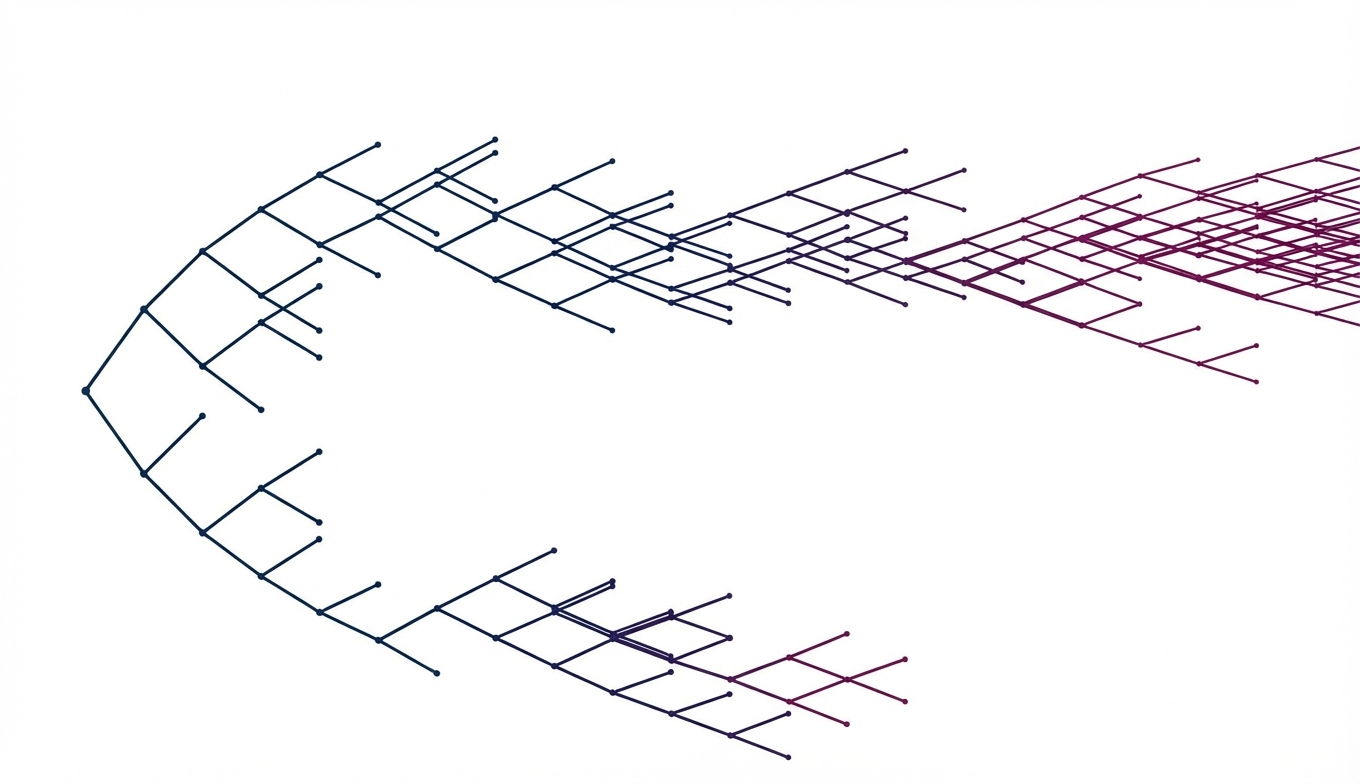
\includegraphics[width=0.7\textwidth]{pictures/simpleGWvis.png}
    \caption*{Realisation of the simple Galton-Watson process with $p=0.58$.}
    \label{fig:example}
\end{figure}




\noindent
Generally, the expected value of a discrete random variable $X$ is defined by
\[
\mathbb{E}(X) = \sum_k \mathbb{P}(X = x_k)\, x_k,
\]
the sum over all possible states $x_k$ in product with their probability of realisation.

Hence, after one generation (with $Z_0 = 1$), we have
\[
\mathbb{E}(Z_1)
= \mathbb{P}(Z_1 = 2)\cdot 2 + \mathbb{P}(Z_1 = 0)\cdot 0.
\]
Replication occurs with probability $p$, resulting in two offspring. So this simplifies to
\[
\mathbb{E}(Z_1) = 2p.
\]

\noindent
By the following argument, we can compute the expected population size
at generation $n$: $\mathbb{E}(Z_n)$.

If we know the value of $Z_n$, then the conditional expectation of the next
generation is
\[
\mathbb{E}(Z_{n+1} \mid Z_n)
= \sum_{i=1}^{Z_n} \mathbb{E}(Z_1)
= 2p\, Z_n.
\]
More generally, if we do not know $Z_n$, the tower property of conditional expectation gives
\[
\mathbb{E}(Z_{n+1})
= \mathbb{E}\bigl( \mathbb{E}(Z_{n+1} \mid Z_n) \bigr)
= \mathbb{E}(2p\, Z_n)
= 2p\, \mathbb{E}(Z_n).
\]

\noindent
Hence,
\[
\mathbb{E}(Z_2) = 2p\, \mathbb{E}(Z_1) = (2p)^2,
\]
\[
\mathbb{E}(Z_3) = 2p\, \mathbb{E}(Z_2) = (2p)^3,
\]
so, induction gives
\[
\mathbb{E}(Z_n) = (2p)^n.
\]





\noindent
From this result, we observe a standard behaviour of branching processes:
\begin{itemize}
    \item If $2p > 1$, then $\mathbb{E}(Z_n)$ grows geometrically with $n$.
    In this case, the branching process is said to be \emph{supercritical}.
    \item If $2p < 1$, then $\mathbb{E}(Z_n)$ decays geometrically with $n$,
    and the branching process is \emph{subcritical}.
\end{itemize}

% INCLUDE SIMULATION GW process in sub and supercrit banching




\begin{figure}[ht]
    \centering
    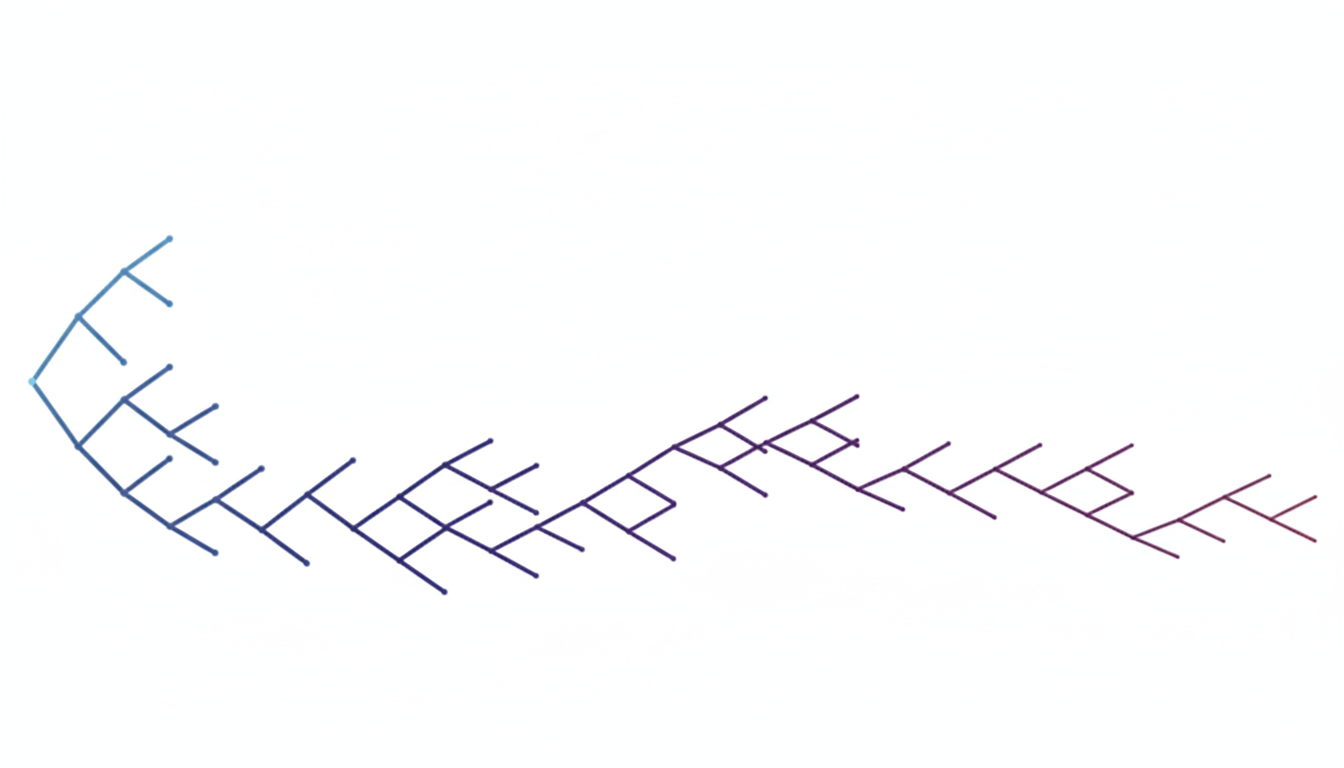
\includegraphics[width=0.7\textwidth]{pictures/subGWvis.png}
    \caption*{Subcritical Galton-Watson realisation with $p=0.47$.}
\end{figure}


\noindent
When $2p = 1$ (that is, $p = 0.5$), the Galton--Watson process is said to be
\emph{critical}. And in this case, the expectation remains constant:
\[
\mathbb{E}(Z_n) = 1^n = 1 \qquad \text{for all } n.
\]

\noindent
However, this does \emph{not} mean that the population survives forever.
Although the expectation remains positive for all finite generations, as in the supercritical case, when $2p = 1$,
ultimate extinction is certain. So the process will eventually fixate at 0, but the expected 
lifetime of the process is infinite.

And this is a curious mathematical result...

Intuitively, it can be understood by the fact that the total lifetime, $T$, of this critical
branching process is distributed according to a power law.

% \begin{figure}[H]
%     \centering
%     \includegraphics[width=0.95\textwidth]{pictures/power_law_extinction.pdf}
%     \caption{Power law distribution of extinction times for the critical Galton--Watson process ($p = 0.5$).
%     (a) The survival probability $S_n = \mathbb{P}(T > n)$ decays as $2/n$ for large $n$.
%     (b) The probability mass function follows $\mathbb{P}(T = n) \sim 2/n^2$, characteristic of a heavy-tailed distribution.
%     Based on $10^5$ simulations.}
%     \label{fig:power_law}
% \end{figure}



\begin{figure}[ht]
    \centering
    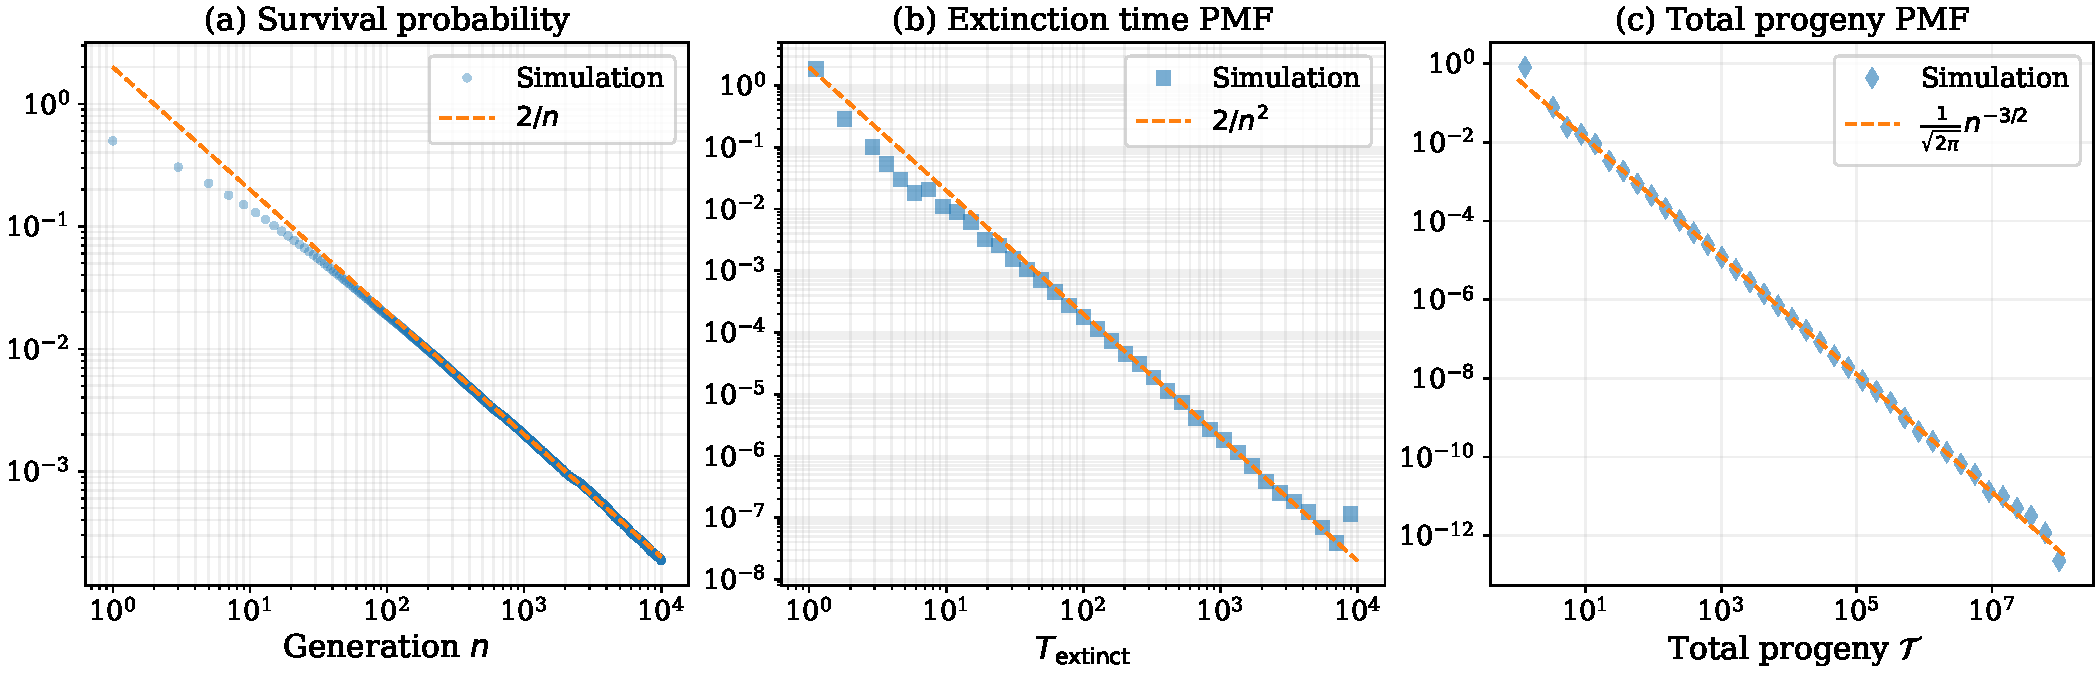
\includegraphics[width=0.98\textwidth]{pictures/power_law_fixed.pdf}
    \caption{
    Power-law behavior in a critical Galton--Watson branching process ($p = 0.5$).\\
    (a) Survival probability
    $S_n  = \mathbb{P}(Z_n > 0)$,
    showing the late generation asymptotic scaling $S_n \sim 2/n$.\\
    (b) Probability mass function of the extinction time
    $T_{\mathrm{extinct}} = \inf\{n : Z_n = 0\}$,
    exhibiting a heavy tail
    $\mathbb{P}(T_{\mathrm{extinct}} = n) \sim 2/n^2$.\\
    (c) Probability mass function of the total progeny
    $\mathcal{T} = \sum_{k \ge 0} Z_k$,
    displaying the classical critical branching asymptotic
    $\mathbb{P}(\mathcal{T} = n) \sim n^{-3/2}$. ($10^6$ realizations).
    }
    \label{fig:power_law}
\end{figure}


\noindent
For such power law distributed variables there is a modestly high chance of extraordinarily large realisations. 
When you compute a sample mean of a power law distributed variable, the more samples you compute, the larger the mean. 
It never converges because the occurance of exceedingly large values pushes the normalised sum higher and higher. 

But aside from this intuative understanding, we will now take an aside to see how this curious result of infinite expected lifetime can be demonstrated.


\subsection{Certainty of extinction and expected lifetime for critical GW branching}

We will fistly derive that extinction is certain in the critical case, then we will go on to demonstrtate that the
expected lifetime of such a process in infinite. 







\subsubsection{Certainty of extinction}


We will see that $u_n$, the probability of extinction by generation $n$, can be computed
using the probability generating function. And it will follow that the probability of ultimate 
extinction will be 1 in both critical and sub-critical branching. $S_n = 1-u_n$ will denote the survival probability,
the liklihood of non-extinction at generation $n$. A computation using $S_n$ will later demonstrate that the expected lifetime, $\mathbb{E}(T)$, is infinite in the critical case.

\vspace{12pt}


\noindent
The probability generating function is defined by
\[
\phi(s) = \mathbb{E}(s^{X}),
\]
for a discrete random variable $X$.

In our case, the offspring distribution is given by $X = Z_1$, and hence
\[
\phi(s) = \mathbb{E}(s^{Z_1}) = p s^2 + (1-p).
\]


\noindent
For the Galton--Watson processes, it is well known that
\[
u_{n+1} = \phi(u_n),
\]
where $u_n$ denotes the probability of extinction by generation $n$.

This relationship can be understood intuitively by considering the fate of the
population after the first generation.

\begin{itemize}
    \item If the process dies in its first step, then extinction has already
    occurred. In this case, the probability of extinction by any generation is
    equal to $1$. This event occurs with probability $1-p$.
    \item If the process replicates in its first step (w/ prob $p$), then the population
    reaches generation $1$ with two individuals. Extinction by generation $n+1$
    then requires both of these fresh lineages to become extinct by their $n$th generation; and this happens w/ prob $u_n^2$.
\end{itemize}

\noindent
Combining these cases yields the recursion
\[
u_{n+1} = (1-p) + p\, u_n^2 = \phi(u_n).
\]
which describes the probability of extinction from one generation to the next. And given the population cannot come 
back to life once it has dies out, $u_n$ will be a non-decreasing sequence bounded above by 1. Conversely, the probability of survival
defined by the complement, $$ S_n = \mathbb{P}(Z_n > 0)  = 1-u_n,$$ will be monotonically decreasing and bounded below by 0, but may converge to a positive value $S_\infty \in [0,1]$.
And to determine how these probabilities behave in the late time limit, we can use the fact that they converge and seek steady state solutions.



Substituting $u_n = 1 - S_n$ into equation (1), we obtain
\[
1 - S_{n+1} = p (1 - S_n)^2 + (1 - p).
\]
Expanding and simplifying gives
\[
S_{n+1}
= 2p S_n - p S_n^2.
\]
To find steady-state solutions, let
\[
S_{n+1} = S_n = S_\infty.
\]
\begin{wrapfigure}{r}{7cm}
    \centering
    \vspace{-10pt} % optional: tighten vertical spacing
    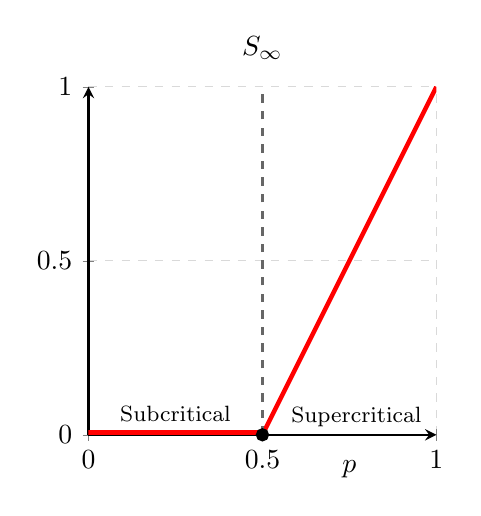
\begin{tikzpicture}
        \begin{axis}[
            width=6cm, height=6cm,
            axis lines=left,
            xlabel={$p$},
            xlabel style={
    at={(axis description cs:0.7,-0.1)},
    anchor=west
},
            xmin=0, xmax=1,
            ymin=0, ymax=1,
            xtick={0, 0.5, 1},
            ytick={0, 0.5, 1},
            grid=major,
            grid style={dashed, gray!30},
            thick,
            title={$S_\infty$}
        ]
            \addplot[red, ultra thick, domain=0:0.5] {0.006};
            \addplot[red, ultra thick, domain=0.5:1] {2*x - 1};
            \draw[dashed, black!60] (axis cs:0.5,0) -- (axis cs:0.5,1);
            \node[font=\footnotesize] at (axis cs:0.25, 0.06) {Subcritical};
            \node[font=\footnotesize] at (axis cs:0.77, 0.05) {Supercritical};
            \addplot[only marks, mark=*, mark size=2pt] coordinates {(0.5,0)};
        \end{axis}
    \end{tikzpicture}
    \vspace{35pt}
\end{wrapfigure}
Then $S_\infty$ satisfies
\[
S_\infty = 2p S_\infty - p S_\infty^2,
\]
or equivalently,
\[
S_\infty \bigl( S_\infty + 1 - 2p \bigr) = 0.
\]


Thus, there are two roots for $S_\infty$ corresponding to two potential steady state solutions.

$$S_\infty = 0 \quad \text{and} \quad S_\infty = 2p - 1$$
But since $S_n$ is a probability, it must lie within the interval $[0,1]$, so when $p < 0.5$, the second root is negative and thus not physically meaningful.
Then, when $p > 0.5$, the probability of survival is positive, given by the larger root, $S_\infty = 2p - 1$. 


\begin{figure}[htbp]
    \centering
    
    % --- Plot 1: p = 0.3 ---
    \begin{subfigure}[b]{0.325\textwidth}
        \centering
        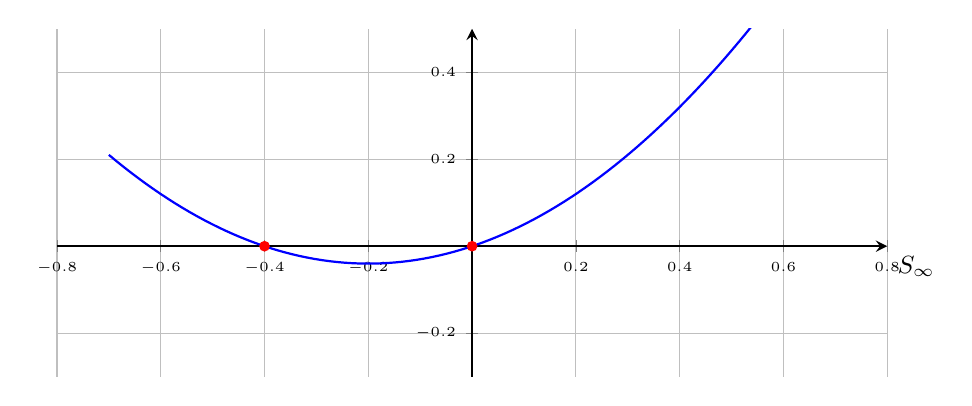
\begin{tikzpicture}
            \begin{axis}[myplotstyle]
                \addplot[blue] {x*(x + 1 - 2*0.3)};
                % Highlight Roots
                \addplot[only marks, mark=*, red, mark size=1.5pt] coordinates {(0,0) (-0.4,0)};
            \end{axis}
        \end{tikzpicture}
        \caption{Subcritical ($p = 0.3$)}
    \end{subfigure}
    \hfill
    % --- Plot 2: p = 0.5 ---
    \begin{subfigure}[b]{0.325\textwidth}
        \centering
        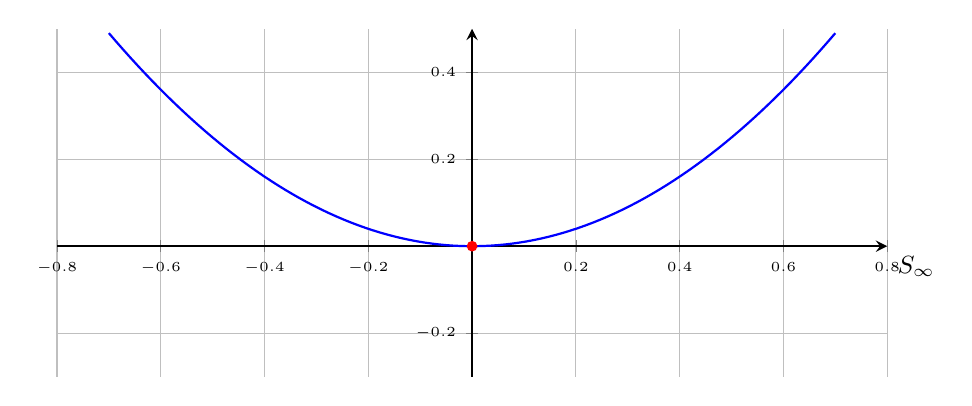
\begin{tikzpicture}
            \begin{axis}[myplotstyle]
                \addplot[blue] {x*(x + 1 - 2*0.5)};
                % Highlight Root (Double root at 0)
                \addplot[only marks, mark=*, red, mark size=1.5pt] coordinates {(0,0)};
            \end{axis}
        \end{tikzpicture}
        \caption{Critical ($p = 0.5$)}
    \end{subfigure}
    \hfill
    % --- Plot 3: p = 0.74 ---
    \begin{subfigure}[b]{0.325\textwidth}
        \centering
        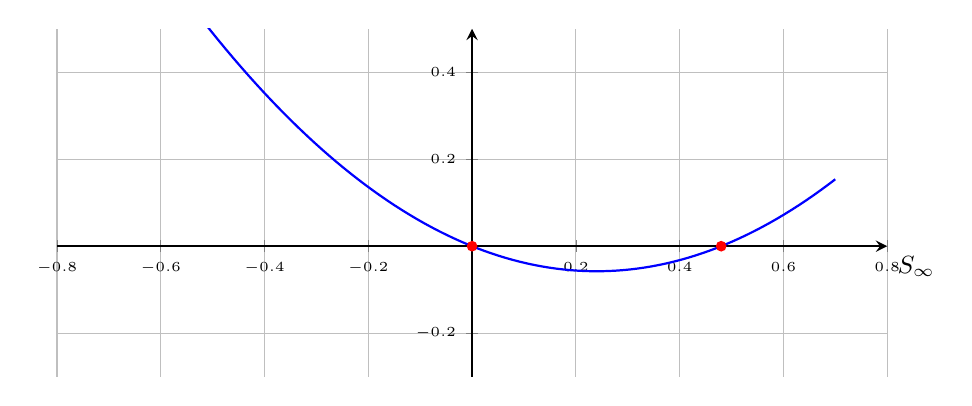
\begin{tikzpicture}
            \begin{axis}[myplotstyle]
                \addplot[blue] {x*(x + 1 - 2*0.74)};
                % Highlight Roots
                \addplot[only marks, mark=*, red, mark size=1.5pt] coordinates {(0,0) (0.48,0)};
            \end{axis}
        \end{tikzpicture}
        \caption{Supercritical ($p = 0.74$)}
    \end{subfigure}

    \caption{Visualizing $S_\infty(S_\infty + 1 - 2p) = 0$. The roots (red dots) represent equilibrium points. At $p=0.5$, the roots collide at the origin, and for $p>0.5$, a stable positive solution $S_\infty = 2p-1$ emerges.}
    \label{fig:phase_transition}
\end{figure}

% \begin{figure}[htbp]
%     \centering
%     \begin{tikzpicture}
%         \begin{axis}[
%             width=6cm, height=6cm, % Square dimensions
%             axis lines=left,
%             xlabel={$p$},
%             ylabel={},
%             xmin=0, xmax=1,
%             ymin=0, ymax=1,
%             xtick={0, 0.5, 1},
%             xticklabels={0, $0.5$, 1},
%             ytick={0, 0.5, 1},
%             grid=major,
%             grid style={dashed, gray!30},
%             thick,
%             xlabel style={anchor=north},
%             ylabel style={anchor=east, rotate=-90},
%             title={$S_\infty$}
%         ]
%             % Subcritical Phase: S_infinity = 0
%             \addplot[red, ultra thick, domain=0:0.5] {0.006};
            
%             % Supercritical Phase: S_infinity = 2p - 1
%             \addplot[red, ultra thick, domain=0.5:1] {2*x - 1};
            
%             % Vertical dashed line at the critical point
%             \draw[dashed, black!60] (axis cs:0.5,0) -- (axis cs:0.5,1);
            
%             % Phase Labels
%             \node[rotate=0, font=\footnotesize] at (axis cs:0.25, 0.06) {Subcritical};
%             \node[rotate=0, font=\footnotesize] at (axis cs:0.77, 0.05) {Supercritical};
            
%             % Critical Point Marker
%             \addplot[only marks, mark=*, mark size=2pt, black] coordinates {(0.5,0)};
%         \end{axis}
%     \end{tikzpicture}
%     \caption{Phase transition diagram showing $S_\infty$ as a function of $p$. The survival probability remains at zero until the critical threshold $p_c = 0.5$, after which it follows $S_\infty = 2p - 1$.}
% \end{figure}

\vspace{10pt}
\noindent
So we have determined that in both the subcritical ($p < 0.5$) and critical ($p = 0.5$) cases, extinction is certain. What about the expected lifetime of the process. How could it be infinite if extinction is certain?




\subsubsection{Expected lifetime}


We are interested in $\mathbb{E}(T)$ when $p = 0.5$, where $T$ denotes the
\emph{extinction time} or the number of generations that the Galton Watson process survives. This is a measure of how many generations the process
survives and is defined as
\[
T = \inf \{ n : Z_n = 0 \}.
\]
that is, the smallest generation index $n$ at which the population is no longer positive.
The process continues over generations
\[
0, 1, 2, \dots, T-1,
\]
then fixates to 0, surviving for $T$ generations in total.

To compute the expected time to extinction, we can entertain the following representation.

\[
T = \sum_{n=0}^{\infty} \mathbf{1}_{\{ T > n \}},
\]
where $\mathbf{1}_{\{\text{boolean}\}}$ is the indicator function, evaluated:
\begin{align*}
    \mathbf{1}_{\{ \text{true}\}} &= 1 \\
    \mathbf{1}_{\{ \text{false}\}} &= 0
\end{align*}



\noindent
The sum involving the indicator function $\mathbf{1}_{\{T>n\}}$ counts one unit
for every generation in which the process is alive.

For example, if $T = 5$, then
\[
\mathbf{1}_{\{T>n\}} = 1 + 1 + 1 + 1 + 1 + 0 + 0 + \cdots .
\]

\noindent
Then, to compute the expected value of $T$,
\[
\mathbb{E}(T)
= \mathbb{E}\!\left( \sum_{n=0}^{\infty} \mathbf{1}_{\{T>n\} } \right)
= \sum_{n=0}^{\infty} \mathbb{E}\!\left( \mathbf{1}_{\{T>n\}} \right),
\]
And given
\[
\mathbf{1}_{\{T>n\}} =
\begin{cases} 
1, & \text{if } T>n, \quad(\text{alive at } n) \\
0, & \text{otherwise},
\end{cases}
\]
with
\[
\mathbb{E}\!\left( \mathbf{1}_{\{T>n\}} \right)
= \mathbb{P}(T>n).
\]
\noindent
$T>n$ is equivalent to $Z_n>0$; the process is still
alive at generation $n$. Therefore,
\[
\mathbb{E}(T)
= \sum_{n=0}^{\infty} \mathbb{P}(Z_n>0).
\]

\noindent
In other words, with $S_n = \mathbb{P}(Z_n>0)$ being the survival probability ay generation $n$,
\[
\mathbb{E}(T) = \sum_{n=0}^{\infty} S_n.
\]

\noindent
Here lies an apparent paradox. We have already established that extinction is certain in the critical case, so $S_n \to 0$ as $n \to \infty$.
Yet the expected time to extinction is infinite, and $\mathbb{E}(T)$ is the sum of $S_n$ which collapses to 0.

Explaining this will require the curious fact that the harmonic series sum is non-convergent.
$$\sum_{n=1}^{\infty} \frac{1}{n} = \infty$$

\begin{figure}[H]
    \centering
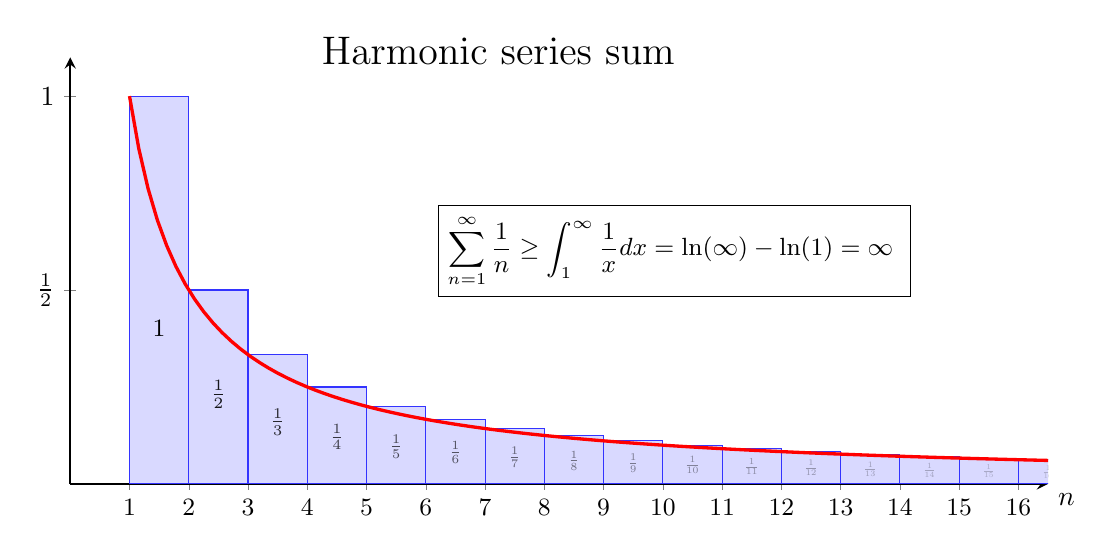
\begin{tikzpicture}
    \begin{axis}[
        axis lines = middle,
        xmin = 0, xmax = 16.5,
        ymin = 0, ymax = 1.1,
        xlabel = {$n$},
        ylabel = {},
        xtick = {1, 2, 3, 4, 5, 6, 7, 8, 9, 10, 11, 12, 13, 14, 15, 16}, 
        ytick = {0.5, 1},
        yticklabels = {$\frac{1}{2}$, $1$},
        axis line style = {thick},
        width = 14cm, 
        height = 7cm,
        every axis x label/.style={at={(current axis.right of origin)}, anchor=north west},
        every axis y label/.style={at={(current axis.above origin)}, anchor=south east},
        title = {Harmonic series sum},
        xticklabel style={font=\small},
    title style={yshift=-12pt, xshift=-22pt, font=\Large},
    ]

        % 1. Harmonic Sum as Rectangles
        \addplot[
            fill=blue!15,
            draw=blue!80,
            ybar interval,
            samples at={1, 2, ..., 17} 
        ]
        {1/x} \closedcycle;

        % 2. Asymptotic Integral Curve (1/x)
        \addplot[
            red,
            domain=1:16.5,
            samples=100,
            very thick
        ]
        {1/x};

        % 3. Automated Loop for Labels
    \node[opacity=1.00, scale=1.00] at (axis cs: 1.5, 0.40) {\small $1$};

\node[opacity=0.90, scale=0.95] at (axis cs: 2.5, 0.23) {\small $\frac{1}{2}$};

\node[opacity=0.82, scale=0.90] at (axis cs: 3.5, 0.16) {\small $\frac{1}{3}$};

\node[opacity=0.75, scale=0.85] at (axis cs: 4.5, 0.121) {\small $\frac{1}{4}$};

\node[opacity=0.68, scale=0.80] at (axis cs: 5.5, 0.097) {\small $\frac{1}{5}$};

\node[opacity=0.62, scale=0.75] at (axis cs: 6.5, 0.081) {\small $\frac{1}{6}$};

\node[opacity=0.56, scale=0.70] at (axis cs: 7.5, 0.069) {\small $\frac{1}{7}$};

\node[opacity=0.50, scale=0.66] at (axis cs: 8.5, 0.060) {\small $\frac{1}{8}$};

\node[opacity=0.45, scale=0.62] at (axis cs: 9.5, 0.053) {\small $\frac{1}{9}$};

\node[opacity=0.40, scale=0.58] at (axis cs: 10.5, 0.0485) {\small $\frac{1}{10}$};

\node[opacity=0.36, scale=0.55] at (axis cs: 11.5, 0.044) {\small $\frac{1}{11}$};

\node[opacity=0.32, scale=0.52] at (axis cs: 12.5, 0.041) {\small $\frac{1}{12}$};

\node[opacity=0.28, scale=0.50] at (axis cs: 13.5, 0.037) {\small $\frac{1}{13}$};

\node[opacity=0.25, scale=0.48] at (axis cs: 14.5, 0.0355) {\small $\frac{1}{14}$};

\node[opacity=0.22, scale=0.46] at (axis cs: 15.5, 0.033) {\small $\frac{1}{15}$};

\node[opacity=0.20, scale=0.44] at (axis cs: 16.5, 0.031) {\small $\frac{1}{16}$};




     
        % 4. Annotation Box
        \node[draw, fill=white, align=left, font=\small] at (axis cs: 10.2, 0.6) {  
            $\displaystyle \sum_{n=1}^{\infty} \frac{1}{n}  \ge \int_{1}^{\infty} \frac{1}{x} dx = \rm{ln}(\infty) - \rm{ln}(1) = \infty$
        };

    \end{axis}
\end{tikzpicture}
\caption{The harmonic series sum diverges. The sum of the areas of the blue rectangles (left) exceeds the area under the red curve (right), which diverges as $x \to \infty$. Thus, $\sum_{n=1}^{\infty} \frac{1}{n} = \infty$. This fact will be used to show that the expected time to extiction in the critical galton watson process is infinite.}
\end{figure}


\noindent
To see how, we first turn our attention to the iterative formula for $S_n$:
\[
S_{n+1} = 2p S_n - p S_n^2.
\]
In the critical case, $p = 0.5$, this becomes
\[
S_{n+1} = S_n - \tfrac{1}{2} S_n^2.
\]
Rearranging gives
\[
S_{n+1} - S_n = -\tfrac{1}{2} S_n^2.
\]
Then, if we consider the late generation limit, $n \gg 1 $, the unit 1 can be considered as a diminishingly small increment compared to $n$, and because of this, the above equation tends to meet the definition of a derivative:

$$\frac{S_{n+1} - S_n}{1} \rightarrow \frac{\mathrm{d}S(n)}{\mathrm{d} n}  = -\tfrac{1}{2} S(n)^2.$$


\noindent
So as $n\to\infty$, the evolution of $S_n$ is increasingly well approximated by this ODE, and thus by its general solution, 
$$S(n) = \frac{2}{n + \text{const.}}$$
Hence, 
\begin{equation}
S_n \sim \frac{2}{n}
\qquad \text{as } n \to \infty, \label{twoovrn_sn}
\end{equation}
which is supported by the numerical simulation results displayed in Figure \ref{fig:power_law}(a).

Then, coming back to the question of expected lifetime in the the critical case, we find that the sum tends towards 2 times the harmonic series in the late generation limit:

$$\mathbb{E}(T) = \sum_{n=0}^{\infty} S_n \sim \sum_{n=1}^{\infty} \frac{2}{n}.$$
And given $S_n$ is always positive and that the harmonic series sum diverges, it can be concluded that $E(T)$ diverges too. Thus, the expected lifetime of the critical Galton-Watson process is infinite, despite the certainty of extinction.






\section{Limiting Conditional Mean $\mathbb{E}(Z_n|Z_n>0) = 1/A(p)$}


With $0 \le p \le \tfrac12$ (and non-degenerate offspring law), the Galton--Watson process becomes extinct almost surely. For the constant $A(p)$ we restrict to the open subcritical interval $p\in[0,\tfrac12)$, where $A(p)\in(0,\tfrac12]$. But picture this: You 
initiate a large number of such branching chains with equal $p\leq 0.5$, and watch as they simultaneously progress. 
Many will die out early, but some may persist for many generations. Here, we will consider the behaviour of those realisations
which outlive the majority. 

Specifically, we will aim to compute $\mathbb{E}(Z_n|Z_n>0)$ for $n\to \infty$, the conditional limiting mean 
of non-extinct populations, and we will see that it becomes stationary.

\vspace{20pt}

\noindent
To begin, we can decompose the expectation of population size into the two conditional expectations of persistence and cessation: 

$$\mathbb{E}(Z_n) = \mathbb{E}(Z_n|Z_n>0)\cdot\mathbb{P}(Z_n>0) + \mathbb{E}(Z_n|Z_n=0)\cdot\mathbb{P}(Z_n=0).$$

\noindent
Since $\mathbb{E}(Z_n|Z_n=0) = 0$, and $\mathbb{P}(Z_n > 0) = S_n$, this simplifies to

$$\mathbb{E}(Z_n) = \mathbb{E}(Z_n|Z_n>0)\cdot S_n.$$
Hence,
$$\mathbb{E}(Z_n|Z_n>0) = \frac{\mathbb{E}(Z_n)}{S_n}.$$
Then, we know that $\mathbb{E}(Z_n) = (2p)^n$, so
$$\mathbb{E}(Z_n|Z_n>0) = \frac{(2p)^n}{S_n}.$$
And we understand what happens to $(2p)^n$ for large $n$. But what about $S_n$? It may go to 0 in the limit, but how does it get there, and what will this say about the conditional mean?




Recall the recursion
\[
S_{n+1} = 2p\, S_n - p\, S_n^2.
\]
Because $S_n \to 0$, for growing generation count the quadratic term $p S_n^2$ diminishes faster than the
linear term. Consequently, at large $n$ the recursion is increasingly well approximated by
\[
S_{n+1} \sim 2p\, S_n.
\]
And thus there exists a constant $A(p)\in(0,\tfrac12]$, depending on $p$ but not on $n$, such that
\begin{equation}
\label{eq:Sn-asymp}
S_n \sim A(p)\,(2p)^n
\qquad\text{as }n\to\infty,
\end{equation}
or equivalently
\begin{equation}
\label{eq:Ap-def-main}
 A(p) = \lim_{n \to \infty} \frac{S_n}{(2p)^n}.
\end{equation}
(The limit of $S_n$ itself is $0$ for $p<\tfrac12$; one must not write $\lim S_n = A(p)(2p)^n$ as an ordinary limit identity.)
The constant $A(p)$ absorbs the cumulative effect of the quadratic terms in the survival recurrence before the linear regime dominates.
And it follows that the conditional mean in the late generation limit is given by
\[
 \lim_{n\to\infty} \mathbb{E}(Z_n | Z_n > 0) = \lim_{n \to \infty} \frac{(2p)^n}{S_n} = \frac{1}{A(p)}.
\]
So because $A(p)$ is constant, the limiting conditional mean is also constant; it may also be referred to as the quasi-stationary mean population.

But the constant $A(p)$ is still something of a mystery. As we will see, computing an analytic formula is not straightforward. 

\section{Attempting to compute $A(p)$}

We can compute approximate values of A(p) numerically by iterating $S_{n+1} = f(S_n)$ many times to find very near stationary 
values of $S_n$ at $n \gg 1$. Then, computing $S_{n_{\text{large}}} / (2p)^{n_{\text{large}}}$ gives a value approximating $A(p)$ for that $p$. 
Repeating this over a range of probabilities can plot a curve of $A(p)$ for $p\in[0, 0.5)$. And this works reasonably well most of the time. But not when $p$ is from very close to $p=0.5$, because as $p\to0.5$, the required $n$
for $S_n$ to reach near stationarity grows impractically large.


No elementary closed form for $A(p)$ is known. During the project, a number of approaches were tried, for example:

\begin{itemize}
    \item Continuum approximations of the recurrence $S_{n+1}=f(S_n)$ by an ODE in generation number;
    \item Symbolic regression / genetic search for a closed expression fitted to numerical samples of $A(p)$.
\end{itemize}
None produced a satisfactory elementary formula. Sections below record partial analytic gains (product representation, near-critical asymptotics). The link to the Koenigs function of the logistic map, and a careful account of the obstruction to an elementary closed form, are given in Sections~\ref{sec:koenigs-link}--\ref{sec:ncf-main}. Exceptional elementary linearisations exist at logistic parameters $r=2$ and $r=4$, but those multipliers lie \emph{outside} the subcritical branching window $r=2p\in[0,1)$; see Appendix~\ref{app:integrable}.

\subsection{Derivation of $A(p)$ as an infinite product}
We may not have found a closed formula for $A(p)$, but here is a derivation of $A(p)$ represented using an infinite product.

Taking, the nonlinear map for $S_k$,
$$S_{n+1} = 2pS_n -pS_n^2.$$
To begin, substitute $S_n = 2w_n$. Then
\begin{align*}
2w_{n+1}
&=
2p\cdot(2w_n)-p\cdot(2w_n)^2
=
4p\,w_n-4p\,w_n^2,
\end{align*}
so with $r=2p$,
\begin{equation}
\label{eq:logistic-from-S}
w_{n+1}
=
r\,w_n(1-w_n)
=
f_r(w_n).
\end{equation}
This is the logistic map on the unit interval. For $r\in[0,4]$ it exhibits the familiar period-doubling cascade; subcritical branching uses only the window $r=2p\in[0,1)$.

\begin{figure}[htbp]
    \centering
    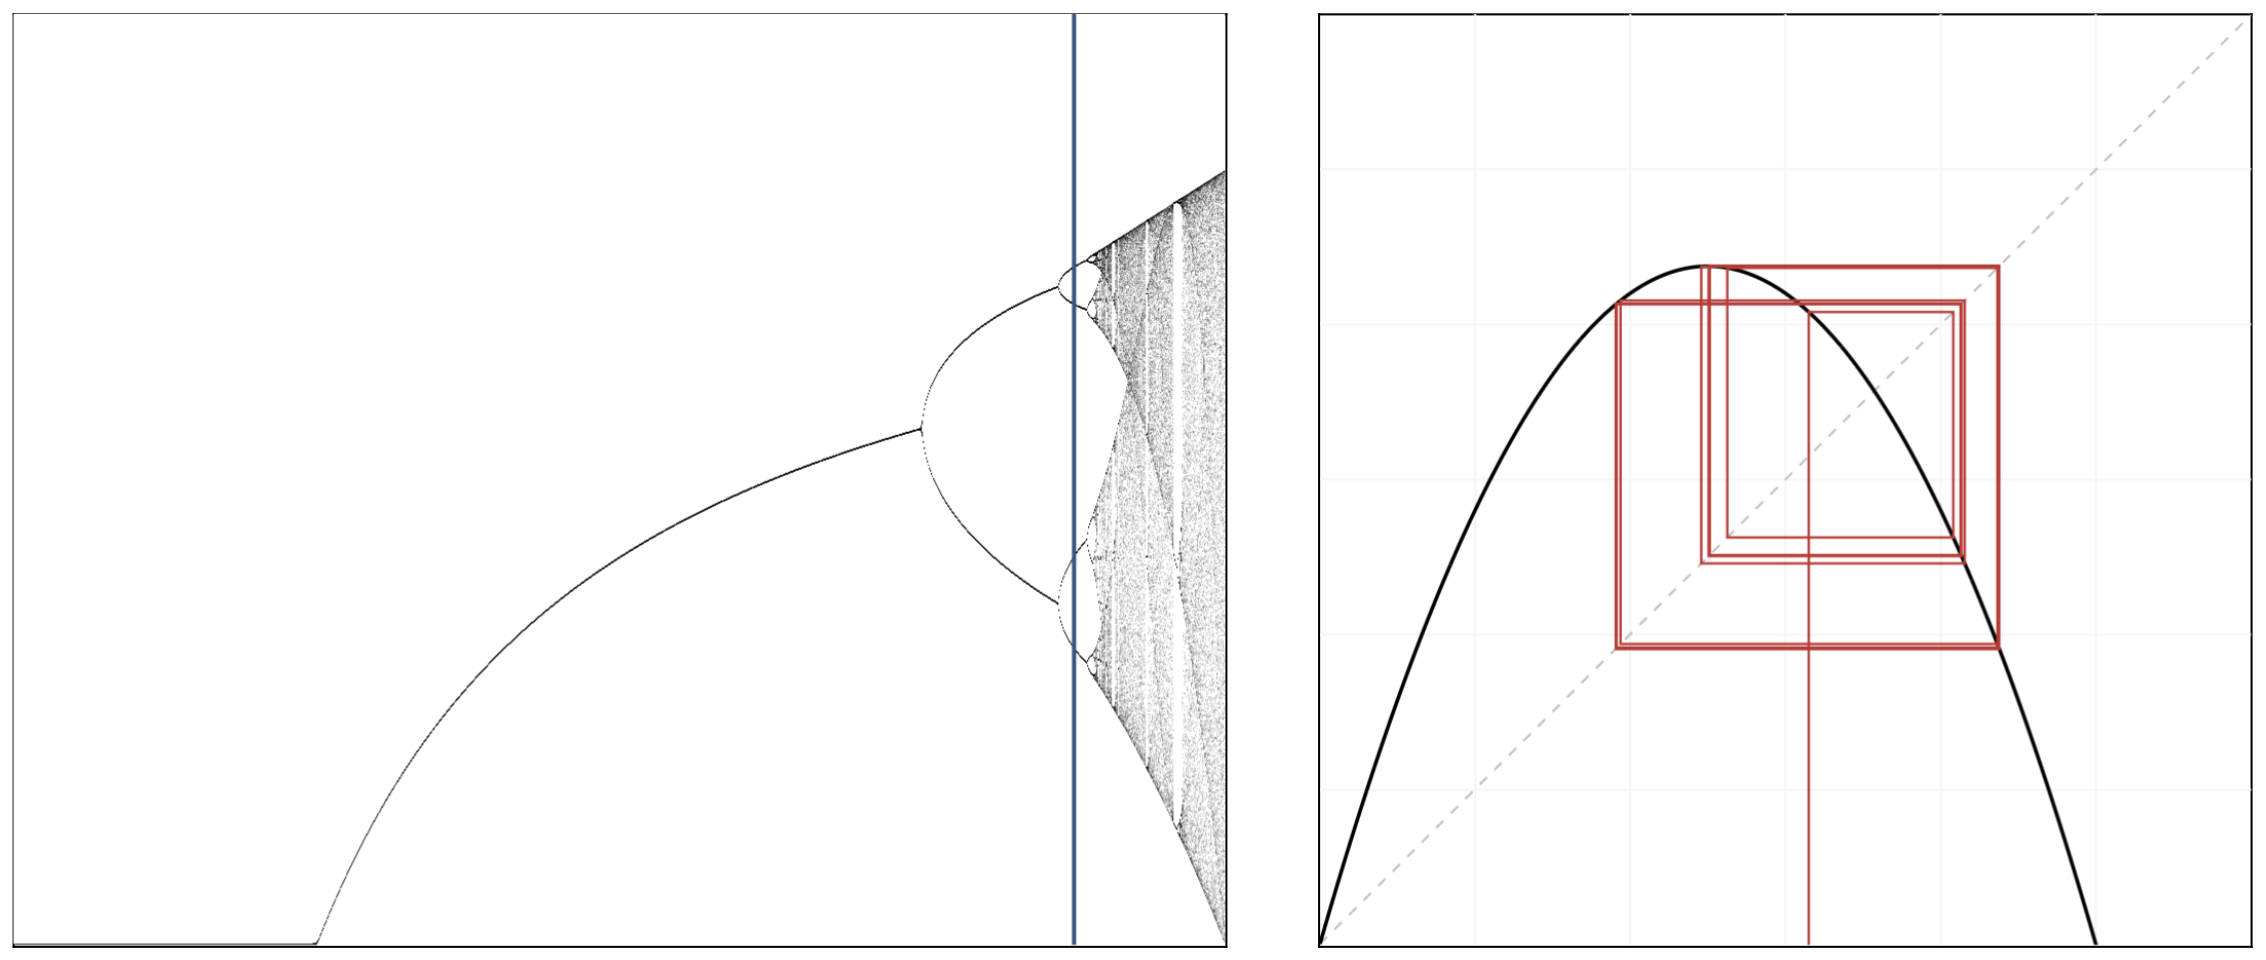
\includegraphics[width=0.8\textwidth]{pictures/period_double.png}
    \caption{Phase diagram of the logistic map that shows the period doubling of stable states, ultimately resulting in chaotic behaviour. Blue sample line on the left at $r=3.5255$, right plot shows a trajectory of the map with the same value of $r$.}
    \label{fig:my_figure}
\end{figure}

\noindent
Now, recall the form of $A(p)$,
$$A(p) = \lim_{n\to\infty} \left(\frac{S_n}{(2p)^n}\right) = 2\lim_{n\to\infty}\left(\frac{w_n}{r^n}\right).$$
Then, because
$$x_n = x_0\left(\frac{x_{1}}{x_{0}}\right)\left(\frac{x_{2}}{x_{1}}\right)\cdots\left(\frac{x_{n-1}}{x_{n-2}}\right)\left(\frac{x_{n}}{x_{n-1}}\right) = x_0\prod^{n-1}_{k=0} \frac{x_{k+1}}{x_k},$$
we can represent an infinite limit as an infinite product: 
$$\lim_{n\to\infty}(x_n) = x_0\prod^\infty_{k=0}\left(\frac{x_{k+1}}{x_k}\right).$$
With $x_n = w_n/r^n$,
$$A(p) = 2\lim_{n\to\infty}\left(x_n\right).$$
And converting this to an infinite product as above, we can simplify the fraction,
\begin{align*}
\frac{x_{k+1}}{x_k} =&\; \frac{\frac{w_{k+1}}{r^{k+1}}}{\frac{w_k}{r^k}} = \frac{w_{k+1}}{w_k}\cdot\frac{r^k}{r^{k+1}}\\
=& \;\;\frac{rw_k(1-w_k)}{w_k}\cdot\frac{1}{r}\\ 
=& \;\; 1-w_k
\end{align*}
leading to
$$A(p) = 2\frac{w_0}{r^0}\prod^\infty_{k=0}(1-w_k)$$
Then, with $w_0 = S_0/2 = 1/2$, and $r^0 = 1$, and pulling out the first ($k=0$) factor,
$$A(p) = \frac{1}{2}\prod^\infty_{k=1}\left(1-w_k\right).$$
And finally, reversing the substitution of $S_n = 2w_n$,
\begin{equation}
\label{eq:prodFormula}
A(p) = \frac{1}{2}\prod_{k=1}^{\infty}\left(1-\frac{S_k}{2}\right).
\end{equation}
So here we have a different formula for $A(p)$ which can be used to progressively compute an aproximation by multiplying successive factors. But this still requires producing the values of $S_n$ by iterating the nonlinear map, so it's not clear that this result brings any material advantage. 


\subsubsection{Convergence of the product}
For $0<w_k<1$, the infinite product $\prod_{k=1}^{\infty}(1-w_k)$ converges to a strictly positive limit if and only if $\sum_{k=1}^{\infty}w_k<\infty$.
From the recurrence $w_{n+1}=r w_n(1-w_n)$ with $0<r<1$ and $0<w_n<1$,
\[
w_{n+1}<r w_n.
\]
By induction $w_n\le w_0 r^n$. Since $0<r<1$, the bound is summable, so $\sum_k w_k<\infty$ and therefore
\[
\prod_{k=1}^{\infty}(1-w_k)
\]
converges to a positive finite value. Combined with the exact product identity, this confirms that the limit defining $A(p)$ is positive and finite for each $p\in(0,\tfrac12)$.


\subsubsection{Advantages of the infinite product formula.}


\subsection{Asymptotic formula for $A(p)$ as $p\to\tfrac12^-$}

Recall
\[
S_{n+1}=2p\,S_n-p\,S_n^2,\qquad S_0=1,
\]
and
\[
\mathbb{E}(Z_n\mid Z_n>0)=\frac{(2p)^n}{S_n}\to\frac{1}{A(p)}
\]
whenever the limit defining $A(p)$ exists. Direct numerical evaluation of $S_n/(2p)^n$ becomes expensive as $p\to\tfrac12^-$, because $A(p)\to0$, the conditional mean diverges, and $S_n$ decays only very slowly. A continuum approximation restores the leading asymptotic.

\paragraph{Exact difference and continuum limit.}
Write $\varepsilon=1-2p\to0^+$, so $p=\tfrac12(1-\varepsilon)$ and $2p=1-\varepsilon$. Then
\begin{equation}
\label{eq:S-diff}
S_{n+1}-S_n
=
(2p-1)S_n-p\,S_n^2
=
-\varepsilon S_n-p\,S_n^2
=
-\varepsilon S_n-\tfrac12 S_n^2+\tfrac{\varepsilon}{2}S_n^2.
\end{equation}
(The linear coefficient is $2p-1=-\varepsilon$.) Treating generation number as continuous for large $n$ and dropping the higher-order $O(\varepsilon S_n^2)$ term yields the Riccati ODE
\begin{equation}
\label{eq:S-ode}
\frac{\mathrm{d}S}{\mathrm{d}n}
=
-\varepsilon S-\tfrac12 S^2.
\end{equation}

\paragraph{Solution via $u=1/S$.}
Set $u=1/S$. Then
\[
\frac{\mathrm{d}u}{\mathrm{d}n}
=
\varepsilon u+\tfrac12,
\]
with integrating factor $e^{-\varepsilon n}$:
\[
\frac{\mathrm{d}}{\mathrm{d}n}\bigl(u e^{-\varepsilon n}\bigr)
=
\tfrac12 e^{-\varepsilon n}.
\]
Hence
\[
u(n)
=
C\,e^{\varepsilon n}-\frac{1}{2\varepsilon},
\qquad
S(n)
=
\frac{1}{C\,e^{\varepsilon n}-\frac{1}{2\varepsilon}}
=
\frac{2\varepsilon}{2\varepsilon C\,e^{\varepsilon n}-1},
\]
for a constant $C>0$ fixed by matching (not by $S_0=1$, since the continuum approximation is only for large $n$).

\paragraph{Matching to $S_n\sim A(p)\,(2p)^n$.}
For small $\varepsilon$, $(2p)^n=(1-\varepsilon)^n\sim e^{-\varepsilon n}$. Late-time survival therefore behaves as
\[
S_n\sim A(p)\,e^{-\varepsilon n}.
\]
From the continuum solution, as $n\to\infty$,
\[
S(n)\sim \frac{1}{C}\,e^{-\varepsilon n},
\]
so $A(p)=1/C$. Matching to the critical decay $S_n\sim 2/n$ in the double limit $\varepsilon\to0$ with $n\varepsilon$ of order one fixes $C\sim 1/(2\varepsilon)$. Consequently
\begin{equation}
\label{eq:Ap-asymp}
A(p)
\sim
2\varepsilon
=
2(1-2p)
=
2-4p
\qquad\text{as }p\to\tfrac12^-.
\end{equation}
Equivalently,
\[
\frac{1}{A(p)}
\sim
\frac{1}{2(1-2p)}.
\]
This agrees at leading order with the continuous-time reciprocal conditional mean under the rate matching $p=\beta/(\beta+\mu)$, namely $(1-p)/(1-2p)\sim 1/(2(1-2p))$. Formula~\eqref{eq:Ap-asymp} is the practical surrogate for $A(p)$ in a thin window below criticality where raw iteration of $S_n$ is costly.

\subsection{Genetic algorithm search attempts}

Before the Koenigs connection was appreciated, a number of methods were tried in search of an elementary formula. 
And one of those was a Genetic algorithm search based regression. The concept is simple: create
50 functions at random, measure how close each one of them is to correctly describing the curve,
then select the best 5 and produce a new population of 50 by creating variations on the best 5. 
Measure the new 50, and repeat this cycle of variation and selection many times over.

When implementing the first vesion, I used a search space of combined polynomials; partly because I 
had a feeling that the solution might show up in that form, and partly because of the relative simplicity
of encoding such functions. 

In the minimal case, a basic polynomial of the standard form can be used. 

$$a_0 + a_1p + a_2 p^2 + a_3 p^3 + a_4 p^4 + \cdots$$
And the "genome" encoding this class of functions would be [$a_0,\dots,a_k$], to some arbirtarily chosen max order $k$.
The initial 50 genomes get produced produced as lists of uniformly random generated real coefficients.
It turns out that many different particular and substantially varying formulas will produce a curve that looks very close to correct, but we wanted the one exact formula...
It occured to me that the true formula may contain only integer or rational coefficients. So an updated version pursued polynomials of the form,


$$\frac{a_0}{b_0} +\frac{a_1}{b_1}p +\frac{a_2}{b_2}p^2 +\cdots+\frac{a_k}{b_k}p^k$$
with $[a_0,\dots,a_k]\in\mathbb{Z}^k$ \& $[b_0,\dots,b_k]\in\mathbb{Z}^k$. Then, after some experiments yielding no definate solution, I also tried extending the formula space to 



$$\frac{\frac{a_0}{b_0} +\frac{a_1}{b_1}p +\frac{a_2}{b_2}p^2 +\cdots+\frac{a_k}{b_k}p^k}{\frac{c_0}{d_0} +\frac{c_1}{d_1}p +\frac{c_2}{d_2}p^2 +\cdots+\frac{c_k}{d_k}p^k}$$
with genome $[a_0,\dots,a_k,b_0,\dots,b_k,c_0,\dots,c_k,d_0,\dots,d_k]\in\mathbb{Z}^{4k}$.
But after numerous searches, the best that was found merely fit the high precision numerically generated data points quite well. And the formula didn't appear simple enough to represent a probably closed solution: 

$$\hat A_1(p) = \frac{\frac{1}{2}(1-2p)(1+2p)}{1 + \frac{1}{2}p - \frac{5}{2}p^2 - \frac{6}{5}p^3 + \frac{6}{5}p^4}$$
It started to become increasingly apparent that a huge number of very different formulas can behave almost identically in a given range. 

$\hat A_1(p)$ does pass through (0, 0.5) \& (0.5, 0) and form a pretty good approximation of the curve visually. Though it does not pass the horizontal axis with the correct gradient of -4 that we know from the asymptotic analysis above. Instead, it passes (0.5, 0) with a gradient of -3.636.

\vspace{10pt}
\noindent
Two years after setting this work aside, I decided to have another go at using an evolutionary regression method like this one to find $A(p)$.
It was just starting to become apparent that no formula exists, but I had another go anyway. This time with the option of using AI tools to write a 
more sophisticated symbolic tree-search program with leveraged time and effort. This new version is capable of searching a space of progressively nested elimentary functions of all kinds. Although, of course, a similar
conclusion was reached: many functions of varying form will closely resemble the target curve, but no satisfactory simple formula emerged, even on favouring solutions of less component parts.

Below are a couple of generated curves selected arbirtatily from the sea of similarly performing candidates.

\begin{multline*}
\hat A_2(p) = 0.31696448624690005 \,
\ln\!\Biggl(
\Biggl|
\cos\!\biggl(
\sqrt{
\biggl|
\sqrt{
\biggl|
\frac{p/p}{| 3.19801133824532 |}
\biggr|
}
\biggr|
} \\
+
\biggl(
\sin\!\Bigl(
\cos\!\bigl(
|p| \,
(0.621865696665606 - p)\,
\cos(e^{e^{p}})
\bigr)
\Bigr)
+
e^{\ln(|p|)}
\biggr) p
\biggr)
\Biggr|
\Biggr)
+ 0.5982282661889831
\end{multline*}

\noindent
As you can see, there are some redundancies in the formula above such as $p/p$. These are introduced by the program sort of like neutral mutations in biological evolution having no effect on fitness. Below is the same formula but with these removed.

% Second equation - use multline
\begin{multline*}
\hat A_2(p) = 0.31696448624690005 \,
\ln\!\Biggl(
\Biggl|
\cos\!\biggl(
\left( \frac{1}{3.19801133824532} \right)^{\!1/4} \\
+
p \biggl[
\sin\!\Bigl(
\cos\!\bigl(
|p| (0.621865696665606 - p)\,
\cos(e^{e^{p}})
\bigr)
\Bigr)
+
|p|
\biggr]
\biggr)
\Biggr|
\Biggr)
+ 0.5982282661889831
\end{multline*}

\noindent
The next one is a bit more concise:

% Third and fourth equations fit on one line as-is
\[
\hat A_3(p)  = \frac{-0.616647881739505 \, e^{-0.552605335919693 \, e^p}}{\sin(\cos p) - |p|} + 0.921964323679771
\]

PLOTIT

\noindent
But a big problem with this formula and others produced by this program is that they either do not pass through the horizontal axis at (0.5,0) or they do not have the correct gradient of -4 at the critical point. And these discrepancies cause big inaccuracies when computing the quasistationary mean with $1/A$ as $p$ approaches 0.5 and $A$ draws ever closer to 0. So whilst making the program which plots many Galton-Watson trajectories along with the horisontal red dashed line indicating the QS mean, I played around with a combined apprach seen in $\hat A_4(p)$ which aims to correct the near critical behaviour with the asymptotic formula. 


\[
\hat A_4(p) = 
\begin{cases}
-0.04011483983619545\, e^{e^{2p}} + 0.6079994336528085, & p < 0.499962,\\[2mm]
2 - 4p, & p \ge 0.499962.
\end{cases}
\]


\noindent
This essentially worked, but I found a better solution in a combination of the numerically generated values in combination with the aysmptotic $2-4p$ in a narrow region of $p$ close to 0.5.



\section{Relationship to the Koenigs function}
\label{sec:koenigs-link}

We now make precise the link between $A(p)$ and the classical linearisation of the logistic map, and then import the content of the ``no closed form'' analysis for the conjugacy on $r\in(0,1)$.

\subsection{From the survival recurrence to the logistic map}

Recall
\[
S_{n+1}=2p\,S_n-p\,S_n^2,\qquad S_0=1,
\]
and $A(p)=\lim_{n\to\infty}S_n/(2p)^n$. Setting $S_n=2w_n$ and $r=2p$ yields the logistic iteration
\begin{equation}
\label{eq:logistic}
w_{n+1}=f_r(w_n),\qquad f_r(w)=r w(1-w),\qquad w_0=\tfrac12,
\end{equation}
with $r\in[0,1)$ throughout the subcritical regime. Then
\begin{equation}
\label{eq:A-from-w}
A(p)=2\lim_{n\to\infty}\frac{w_n}{r^n}.
\end{equation}

\subsection{Koenigs linearisation}

\begin{definition}[Koenigs function for the logistic map]
\label{def:koenigs}
Let $f_r(z)=r z(1-z)$ with multiplier $r$ at the fixed point $0$ satisfying $0<|r|<1$. There exists a unique holomorphic map $\psi_r$, defined in a neighbourhood of $0$, such that
\begin{equation}
\label{eq:schroder}
\psi_r\bigl(f_r(z)\bigr)=r\,\psi_r(z),\qquad \psi_r(0)=0,\qquad \psi_r'(0)=1.
\end{equation}
Equivalently,
\begin{equation}
\label{eq:koenigs-limit}
\psi_r(z)=\lim_{n\to\infty} r^{-n} f_r^{\circ n}(z)
\end{equation}
uniformly near the origin \cite{Koenigs1884}. The normalisation $\psi_r'(0)=1$ is equivalent to $\psi_r(z)/z\to1$ as $z\to0$.
\end{definition}

\begin{figure}[H]
\centering
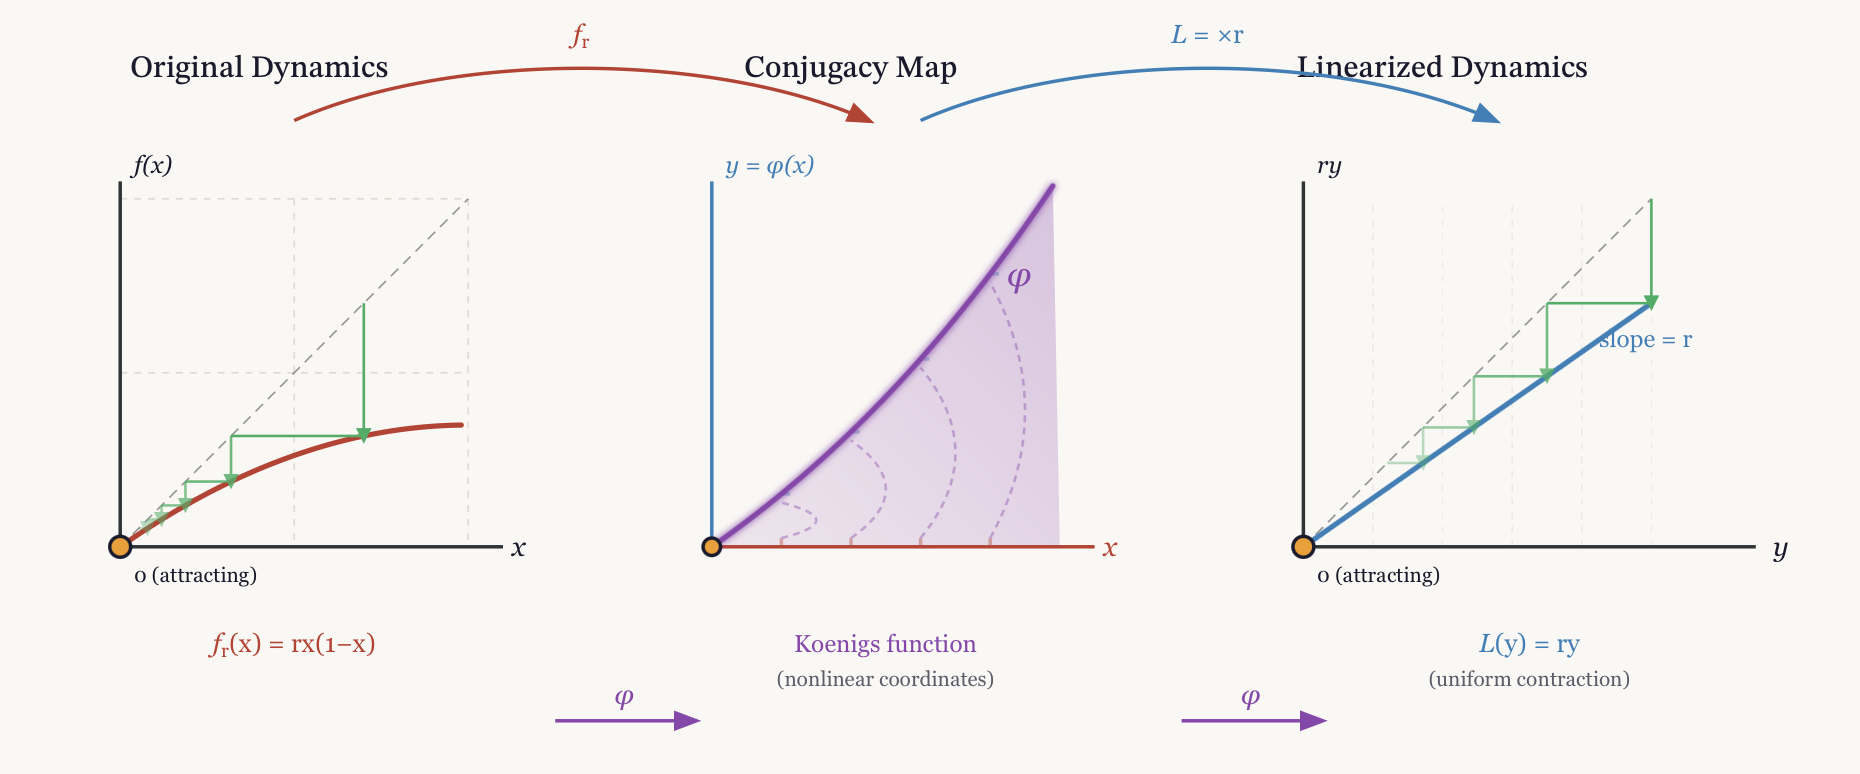
\includegraphics[width=0.78\textwidth]{figures/figure2_koenigs_linearization.png}
\caption{Schematic of Koenigs linearisation: $f_r$ is conjugate, via $\psi_r$, to multiplication by $r$ near the origin.}
\label{fig:koenigs-schematic}
\end{figure}

\subsection{The identity $A(p)=2\lim r^{-n}f_r^{\circ n}(\tfrac12)$}

The local Koenigs function is initially defined only in a neighbourhood of $0$. For $r\in(0,1)$ the origin is attracting on the real line and the interval $(0,1)$ lies in its real basin: starting from $w_0=\tfrac12$, one has $w_n\to0$. On that basin the limit
\begin{equation}
\label{eq:basin-koenigs}
\Psi_r(w_0)
:=
\lim_{n\to\infty} r^{-n} f_r^{\circ n}(w_0)
\end{equation}
exists and agrees with the local conjugacy near $0$ (where $\psi_r'(0)=1$ means $\psi_r(w)/w\to1$ as $w\to0$, so $\psi_r(w_n)/r^n\sim w_n/r^n$). Along the orbit, whenever $w_n$ lies in the local domain,
\[
\psi_r(w_0)=\frac{\psi_r(w_n)}{r^n};
\]
passing to the limit yields $\Psi_r(w_0)=\lim w_n/r^n$. With $w_0=\tfrac12$ and \eqref{eq:A-from-w},
\begin{equation}
\label{eq:A-koenigs}
A(p)
=
2\Psi_r\bigl(\tfrac12\bigr)
=
2\lim_{n\to\infty} r^{-n} f_r^{\circ n}\bigl(\tfrac12\bigr),
\qquad r=2p\in[0,1).
\end{equation}
We write $A(p)=2\psi_r(\tfrac12)$ as a shorthand for this basin value of the Koenigs conjugacy, not as a naive evaluation of a power series beyond its guaranteed disc of convergence.

Thus every question about an elementary closed form for $A(p)$ is tied to the nature of that conjugacy at multiplier $r=2p$.

\section{No elementary closed form for the conjugacy when $r\in(0,1)$}
\label{sec:ncf-main}

This section makes the obstruction precise, and delimits exactly what it does and does not assert. The logical skeleton is short:
(i) every elementary function satisfies an algebraic differential equation;
(ii) differential algebraicity survives compositional inversion;
(iii) by a theorem of Becker and Bergweiler, a solution of Schr\"oder's equation for a rational map of degree at least two can be differentially algebraic only when the underlying fixed point is \emph{repelling};
(iv) for $r\in(0,1)$ the fixed point $0$ of $f_r$ is attracting.
Hypertranscendence of $\psi_r$ for every subcritical parameter follows at once --- with no exceptional cases to exclude, because the attracting window contains no candidates at all. We then explain, with equal care, why this theorem does \emph{not} by itself settle the status of the individual numbers $A(p_0)$ or of the map $p\mapsto A(p)$, and we record the numerical evidence bearing on those.

\subsection{Differential algebraicity, hypertranscendence, elementarity}

\begin{definition}[differentially algebraic; hypertranscendental]
\label{def:da}
A function $g$, holomorphic on a domain (or a formal power series), is \emph{differentially algebraic over $\mathbb{C}(z)$} if there exists a non-zero polynomial $P$ in $n+2$ variables, for some $n\ge0$, with
\[
P\bigl(z,\,g(z),\,g'(z),\,\dots,\,g^{(n)}(z)\bigr)\equiv 0 .
\]
Otherwise $g$ is \emph{differentially transcendental}, or \emph{hypertranscendental}.
\end{definition}

Two closure facts make this the right notion for our purpose.

\begin{lemma}[elementary $\Rightarrow$ differentially algebraic]
\label{lem:elem-da}
Every elementary function in the Liouville sense --- any function reachable from $\mathbb{C}(z)$ by a finite tower of algebraic operations, exponentials and logarithms --- is differentially algebraic. Consequently a hypertranscendental function is not elementary.
\end{lemma}

\begin{proof}[Proof sketch]
Each storey of a Liouvillian tower preserves differential algebraicity: algebraic extensions do so by elimination; if $g$ is differentially algebraic then so are $e^{g}$ and $\log g$, their defining first-order relations combining with the equation for $g$; and the class is closed under field operations and composition. These closure properties are classical; see Rubel's survey \cite{Rubel1989}.
\end{proof}

\begin{lemma}[closure under compositional inversion]
\label{lem:inv-da}
Let $g$ be holomorphic near $0$ with $g(0)=0$ and $g'(0)\neq0$, and let $g^{-1}$ denote its local compositional inverse. Then $g$ is differentially algebraic over $\mathbb{C}(z)$ if and only if $g^{-1}$ is (Moore \cite{Moore1896}; see also Boshernitzan--Rubel \cite{BoshernitzanRubel1986}).
\end{lemma}

\Cref{lem:inv-da} matters because the literature states Schr\"oder-equation results in two equivalent but opposite conventions, and conflating them is an easy way to misquote a theorem. Our $\psi_r$ is the \emph{linearising coordinate}: $\psi_r(f_r(z))=r\,\psi_r(z)$. The function classified by Becker and Bergweiler (and by Ritt before them) is the \emph{linearising parametrisation} $\varphi_r=\psi_r^{-1}$, which satisfies
\begin{equation}
\label{eq:schroder-param}
\varphi_r(r\,t)=f_r\bigl(\varphi_r(t)\bigr),
\qquad
\varphi_r(0)=0,\quad \varphi_r'(0)=1 .
\end{equation}
By \Cref{lem:inv-da}, hypertranscendence of either function transfers to the other.

\subsection{The Becker--Bergweiler theorem, stated precisely}

The result we need is the 1995 classification of differentially algebraic Schr\"oder functions \cite{Becker1995}; we quote it in the form given in Fernandes' survey of the Schr\"oder, B\"ottcher and Abel equations \cite[Thm~3.1]{Fernandes2021}.

\begin{theorem}[Becker--Bergweiler \cite{Becker1995}; as restated in {\cite[Thm~3.1]{Fernandes2021}}]
\label{thm:BB-main}
Let $R$ be a rational map of degree at least two with $R(0)=0$ and multiplier $s=R'(0)$, where $s\neq0$ and $s$ is not a root of unity (for $|s|=1$ the Schr\"oder function is understood as a formal series). Let $\varphi$, normalised by $\varphi(0)=0$ and $\varphi'(0)=1$, solve $\varphi(st)=R(\varphi(t))$. If $\varphi$ is differentially algebraic over $\mathbb{C}(t)$, then:
\begin{enumerate}[label=\textup{(\roman*)}]
\item the fixed point $0$ is \emph{repelling}, $|s|>1$; and
\item $\varphi$ is a M\"obius transformation of one of
\[
\exp(\alpha t^{\rho}),
\qquad
\cos(\alpha t^{\rho}+\beta),
\qquad
\wp(\alpha t^{\rho}+\beta),\ \wp^{2},\ \wp^{3},\ \wp'(\alpha t^{\rho}+\beta),
\]
where $\wp$ is a Weierstrass function, $\rho\in\mathbb{Q}$ is such that the function concerned is meromorphic on $\mathbb{C}$, $\alpha\neq0$, and $\beta$ is a fraction of a period. Correspondingly $R$ is M\"obius-conjugate to $z^{\pm d}$, to $\pm T_d$ (Chebyshev), or to a Latt\`es map.
\end{enumerate}
\end{theorem}

\begin{remark}[lineage and independent corroboration]
\label{rem:lineage}
For $|s|>1$ --- the Poincar\'e-function case --- the classification goes back to Ritt in 1926 \cite{Ritt1926}; Becker and Bergweiler completed the picture for the three classical functional equations at once, and Bergweiler's later account with Aschenbrenner \cite{AschenbrennerBergweiler2015} assigns the exceptional list explicitly to the repelling case. Di~Vizio and Fernandes \cite{DiVizioFernandes2021} have given an independent difference-Galois proof of Ritt's theorem; notably, their Theorems~1.2 and~4.2 assume only that $s$ is neither zero nor a root of unity --- no condition $|s|>1$ --- and show that any differentially algebraic solution of $y(R(x))=s\,y(x)$ (our $\psi$-convention, with no inversion needed) must already satisfy a first-order equation of Ritt type $(y')^{\rho}=B(x)\,y^{\,j}$. The structure underlying \Cref{thm:BB-main} therefore does not hang on a single paper.
\end{remark}

\subsection{Hypertranscendence throughout the subcritical window}

\begin{theorem}[no exceptional parameters in $(0,1)$]
\label{thm:main-ht}
For every $r\in(0,1)$, the Koenigs function $\psi_r$ of $f_r(z)=rz(1-z)$ at $0$ is hypertranscendental over $\mathbb{C}(z)$: it satisfies no algebraic differential equation. In particular, $\psi_r$ is not an elementary function.
\end{theorem}

\begin{proof}
Fix $r\in(0,1)$. The map $f_r$ is rational of degree two, fixes $0$, and its multiplier $s=f_r'(0)=r$ satisfies $0<s<1$; the hypotheses of \Cref{thm:BB-main} hold, with $0$ attracting. Suppose, for contradiction, that $\psi_r$ were differentially algebraic. Its local inverse $\varphi_r=\psi_r^{-1}$ solves the parametrisation form \eqref{eq:schroder-param} with the stated normalisation, and by \Cref{lem:inv-da} it would be differentially algebraic too. \Cref{thm:BB-main}(i) would then force $|r|>1$, contradicting $r\in(0,1)$. Hence $\psi_r$ is hypertranscendental, and non-elementarity follows from \Cref{lem:elem-da}.
\end{proof}

\begin{remark}[the exceptional set inside the window is empty, not merely avoided]
\label{rem:empty}
An earlier form of this argument reasoned through the parameter plane: the affine conjugacy $c(r)=(2r-r^{2})/4$ of \Cref{lem:affine} sends $r\in(0,1)$ to $c\in(0,\tfrac14)$, which avoids the exceptional quadratic parameters $c=0$ (reached at $r=2$) and $c=-2$ (reached at $r=4$, and also at $r=-2$). That observation is true but logically superfluous, and it invites a question it cannot answer --- \emph{is the exceptional list, restricted to the window, complete?} The route through \Cref{thm:BB-main}(i) dissolves the question: the exceptional Schr\"oder functions exist only over \emph{repelling} fixed points, so the attracting window contains no candidates whatsoever, and no enumeration of exceptional parameters is required. Consistently, the classical elementary cases of Appendix~\ref{app:integrable} have multipliers $2$ and $4$ at the linearised fixed point --- both repelling: they are Poincar\'e-type linearisations, and neither can be pressed into service for $r\in(0,1)$.
\end{remark}

\begin{figure}[H]
\centering
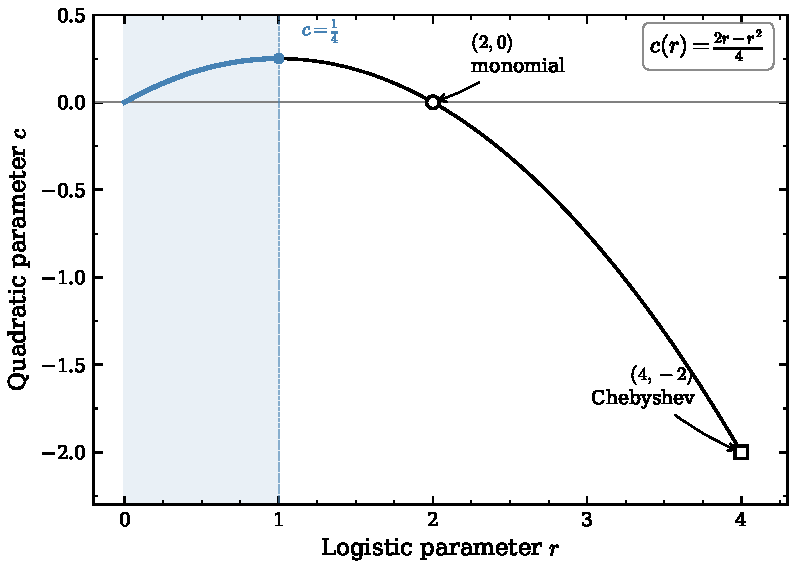
\includegraphics[width=0.72\textwidth]{figures/figure1_parameter_conjugacy.pdf}
\caption{Parameter correspondence $c(r)=(2r-r^2)/4$. The segment $r\in(0,1)$ maps to $c\in(0,\tfrac14)$, disjoint from the integrable values $c\in\{0,-2\}$. In the light of \Cref{rem:empty} this picture is a consistency check rather than the proof: the exceptional linearisations live over repelling fixed points, which the attracting window excludes outright.}
\label{fig:c-of-r}
\end{figure}

\begin{remark}[germ versus basin]
\label{rem:basin}
\Cref{thm:main-ht} concerns $\psi_r$ as an analytic function; the quantity $A(p)=2\Psi_r(\tfrac12)$ of \eqref{eq:A-koenigs} uses its extension to the real basin of attraction, since for $p\ge\tfrac13$ the point $\tfrac12$ lies outside the disc on which Koenigs' series is guaranteed to converge (radius $(1-r)/r$). The extension is by finitely many applications of the functional equation,
\[
\Psi_r(w)=r^{-N}\,\psi_r\bigl(f_r^{\circ N}(w)\bigr)
\quad\text{for $N$ large enough that $f_r^{\circ N}(w)$ enters the germ,}
\]
and an algebraic differential equation, if one held on any subdomain, would persist under this analytic continuation. Hypertranscendence of the germ and of the basin extension are therefore equivalent statements, and the identity \eqref{eq:A-koenigs} is unaffected.
\end{remark}

\begin{figure}[H]
\centering
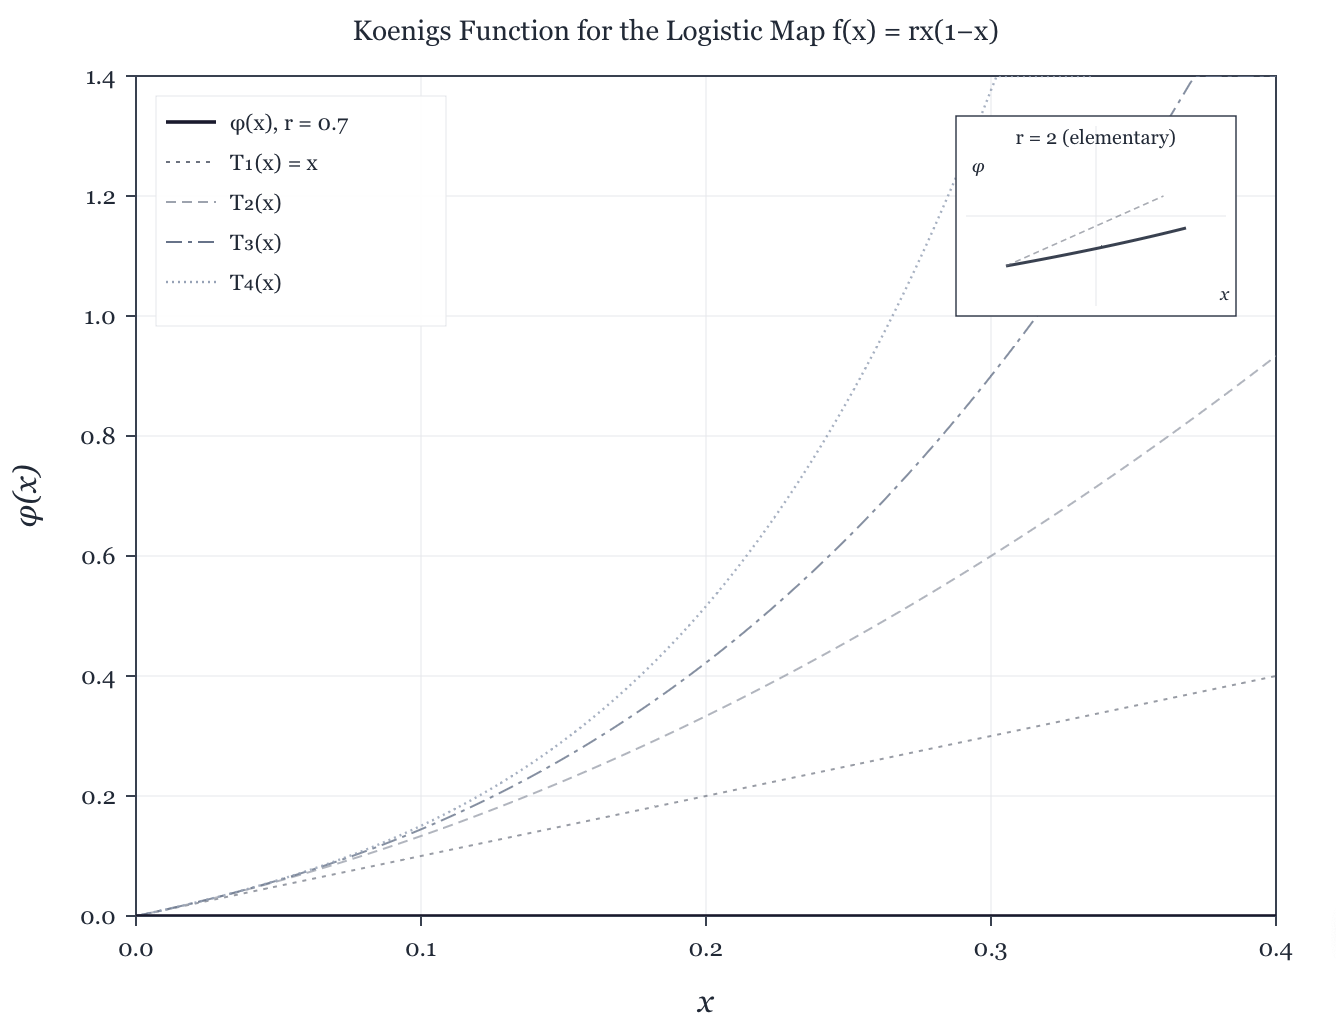
\includegraphics[width=0.72\textwidth]{figures/figure3_numerical_koenigs.png}
\caption{Numerical approximation of a Koenigs function for a logistic multiplier in $(0,1)$, with low-order Taylor polynomials near the origin. Elementary closed forms exist only for exceptional multipliers outside this range (Appendix~\ref{app:integrable}).}
\label{fig:koenigs-numeric}
\end{figure}

\subsection{What the theorem does and does not say about $A(p)$}
\label{subsec:scope}

``Closed form'' must itself be made precise before the claim is stated; at least four inequivalent readings are in play, and a result for one is not a result for another.
\begin{enumerate}[label=\textup{(\Alph*)},leftmargin=*]
\item[\textbf{(V)}] the \emph{value} $A(p_0)$ is elementary or algebraic, for a fixed rational $p_0$;
\item[\textbf{(E)}] the \emph{map} $p\mapsto A(p)$ is an elementary function of $p$;
\item[\textbf{(D)}] the map is \emph{differentially algebraic in $p$}, i.e.\ satisfies some algebraic ODE in $p$;
\item[\textbf{(S)}] the map is expressible via standard special functions ($\Gamma$, $\zeta$, ${}_2F_1$, theta or $q$-series).
\end{enumerate}
\Cref{thm:main-ht} speaks to the function $z\mapsto\psi_r(z)$ at fixed $r$, and licenses exactly this much: \emph{no evaluation of $A(p)$ can be short-circuited through an algebraic differential equation for the lineariser, at any subcritical parameter.} It does not, by itself, decide any of (V), (E), (D) or (S). Two gaps must be stated plainly.

\paragraph{The value gap.}
A hypertranscendental function can take elementary --- even algebraic --- values at individual points: $\Gamma$ is hypertranscendental by H\"older's theorem, yet $\Gamma(\tfrac12)=\sqrt{\pi}$. Nothing so far forbids, say, $A(\tfrac14)$ from being an algebraic number. There \emph{is} a genuine values theorem in this circle of ideas: Becker and Bergweiler proved in 1993 \cite{Becker1993} that the B\"ottcher conjugacy between two polynomials of the \emph{same degree} $d\ge2$ with algebraic coefficients (not linearly conjugate to monomials or Chebyshev polynomials) is transcendental and takes transcendental values at algebraic points; Mahler's method drives the proof (for the method, see Nishioka \cite{Nishioka1996}). One might hope to transfer this to the Koenigs value $\psi_r(\tfrac12)$. It does not transfer, for two independent reasons. \emph{Formally}, the Schr\"oder equation pairs an inner map of degree two with an outer map --- multiplication by $r$ --- of degree one, so the equal-degree hypothesis fails outright. \emph{Structurally}, no easy repair exists: Mahler's method balances doubly-exponential analytic decay along an orbit against comparable height growth, and in the B\"ottcher setting both exponents run like $d^{\,n}$; in the attracting Koenigs setting the orbit $w_n=f_r^{\circ n}(\tfrac12)$ decays only geometrically, $|w_n|\sim A\,r^{n}$, while the heights of the rational numbers $w_n$ still grow doubly exponentially, $h(w_n)\sim C\,2^{\,n}$, and the resulting inequalities run the wrong way at every $n$. Note that the obstruction is \emph{not} the germ/basin issue --- the pullback of \Cref{rem:basin} moves the evaluation point arbitrarily deep into the germ at the cost of a rational factor --- it is the degree structure of the equation itself. The consequence deserves emphasis:
\begin{center}
\emph{transcendence --- indeed, even irrationality --- of $A(p_0)$ is at present not proved\\ for a single rational $p_0\in(0,\tfrac12)$.}
\end{center}

\paragraph{The parameter gap.}
\Cref{thm:main-ht} says nothing about the map $p\mapsto A(p)$: readings (E) and (D) are open. To the best of our knowledge the question is not merely unsolved but unaddressed in the literature. The natural machinery --- the parametrised differential Galois theory of difference equations of Hardouin and Singer \cite{HardouinSinger2008}, designed precisely to detect differential relations in auxiliary directions for linear difference equations such as $\sigma\psi=r\psi$ --- does not apply as it stands, because the derivation $\partial_r$ fails to commute with the substitution operator $\sigma\colon w\mapsto f_r(w)$, which itself moves with $r$. Nor does any feature of the near-critical asymptotics obstruct (E) or (D): logarithmic corrections to \eqref{eq:Ap-asymp} are themselves elementary functions of $\varepsilon$.

\subsection{Inverse-symbolic evidence at eleven rational parameters}
\label{subsec:pslq}

Since the theorems leave (V) open, the value question was attacked directly by integer-relation detection. The values
\[
A(p),\qquad p\in\bigl\{\tfrac1{10},\tfrac18,\tfrac16,\tfrac15,\tfrac14,\tfrac3{10},\tfrac13,\tfrac38,\tfrac25,\tfrac5{12},\tfrac9{20}\bigr\},
\]
were computed to more than $1150$ significant digits by two mechanically independent routes --- the exact product identity \eqref{eq:prodFormula} iterated to convergence, and a pullback of the orbit into the Koenigs germ followed by evaluation of the Koenigs series --- which agreed to at least $1192$ digits at every parameter. Each value was then subjected to a PSLQ battery at $\ge200$-digit effective rigour:
\begin{itemize}
\item \emph{algebraicity}: no integer polynomial relation of degree $\le10$ and coefficient height $\le10^{6}$;
\item \emph{linearity}: no rational linear relation, at height $\le10^{8}$, against the constants $\pi$, $\pi^{2}$, $\ln2$, $\ln3$, $\ln5$, $\gamma$, $\zeta(3)$, $\sqrt2$, $\sqrt3$, $\sqrt5$, $e$, $e^{\pi}$, $\Gamma(\tfrac13)$, $\Gamma(\tfrac14)$ and Catalan's constant (also tested for $1/A$, the quasi-stationary mean itself, and for $A/\varepsilon$);
\item \emph{bilinearity}: no representation $A=L_1/L_2$ with $L_1,L_2$ integer linear forms of height $\le10^{8}$ in a twelve-constant basis (run at $460$ digits);
\item \emph{multiplicativity}: no relation $A=e^{q_0}2^{q_1}3^{q_2}5^{q_3}7^{q_4}\pi^{q_5}$ with rational exponents of height $\le10^{10}$;
\item \emph{cross-parameter}: no rational linear or multiplicative relation linking the eleven values to one another (run at $500$ digits).
\end{itemize}
In all, $123$ tests returned no relation --- indeed no discovery-stage candidate: every PSLQ run terminated on its internal norm bound, so each null carries a genuine ``no relation up to the stated height'' guarantee. Throughout, the precision head-room (digits divided by basis size) exceeded every height cap by at least eight orders of magnitude, so a returned relation would have been meaningful rather than numerical noise.\footnote{Computations in \texttt{mpmath} at working precisions of $310$--$1200$ digits; scripts, the $1150$-digit values, and the full per-test log are archived with the project sources.}

This is finite evidence, and its scope must be stated honestly: it excludes low-complexity closed forms over the tested constants, and nothing more. A closed form over untested constants ($\Gamma(\tfrac17)$, say, or periods of higher-genus curves), or one of height above the caps, would have escaped the search. It is evidence for the conjecture, not a proof.

\subsection{The working claim}

\begin{quote}
\textit{For every fixed $r=2p\in(0,1)$, the Koenigs linearisation $\psi_r$ is hypertranscendental in its own variable (\Cref{thm:main-ht}) --- a theorem, with no exceptional parameters in the attracting window, since differentially algebraic Schr\"oder functions exist only over repelling fixed points. Consequently no elementary expression in $z$ for the conjugacy can be evaluated to produce $A(p)$. Whether individual values $A(p_0)$ are transcendental (or even irrational), and whether the map $p\mapsto A(p)$ is elementary or differentially algebraic in $p$, remain open questions; no closed form under any reading is known, none is expected, and eleven rational values resist inverse-symbolic identification against standard constants at over $200$-digit rigour.}
\end{quote}

Full derivations of the elementary solutions at $r=2$ and $r=4$, and their place inside the Becker--Bergweiler classification, are collected in Appendix~\ref{app:integrable}.

\section{Practical computation of $A(p)$ and $1/A(p)$}
\label{sec:practical}

In the absence of an elementary formula, $A(p)$ is obtained by iteration of $S_{n+1}=2pS_n-pS_n^2$ (or the product \eqref{eq:prodFormula}) for $p$ bounded away from $\tfrac12$, and by the near-critical asymptotic $A(p)\approx 2-4p$ in a narrow window as $p\to\tfrac12^{-}$. A robust hybrid scheme is
\begin{equation*}
A(p)_{\mathrm{prox}}
=
\begin{cases}
\dfrac12\displaystyle\prod_{k=1}^{N}\Bigl(1-\dfrac{S_k}{2}\Bigr), & p<c,\ \ N\gg 1,\\[1em]
2-4p, & c\le p<\tfrac12,
\end{cases}
\end{equation*}
with a cutoff $c$ slightly below $\tfrac12$ (e.g.\ $0.4999$). This restores accurate quasi-stationary means $1/A(p)$ even where raw iteration becomes expensive.

\section{Conclusion}

The constant $A(p)$ organises the quasi-stationary mean of subcritical binary Galton--Watson branching. It is well defined, computable, and linked to the basin Koenigs value $A(p)=2\lim r^{-n}f_r^{\circ n}(\tfrac12)$ at multiplier $r=2p$. For every $r\in(0,1)$ that conjugacy is hypertranscendental in its own variable (\Cref{thm:main-ht}) --- a theorem with no exceptional parameters in the attracting window, since differentially algebraic Schr\"oder functions exist only over repelling fixed points --- and this explains the failure of every elementary closed-form search, while leaving $A(p)$ fully usable for analysis and numerics. What the theorem does not decide is flagged with equal care: transcendence (even irrationality) of individual values $A(p_0)$, and the elementarity or differential algebraicity of the map $p\mapsto A(p)$ in $p$, are open --- the former because the 1993 Becker--Bergweiler values theorem is confined to equal-degree B\"ottcher pairs and does not transfer, the latter because the question appears nowhere in the literature. Eleven rational values nonetheless resist all inverse-symbolic identification at over $200$-digit rigour. The exceptional elementary linearisations at $r=2$ and $r=4$ (both repelling) lie outside the branching window; their derivations, and their place inside the classification, appear in the appendix.

\clearpage
\appendix

\section{Elementary Koenigs functions at $r=2$ and $r=4$}
\label{app:integrable}

These cases lie outside subcritical branching ($r=2p<1$) but complete the classical picture of integrable logistic linearisations. The derivations follow the closed-form note integrated into this document.

\subsection{Case $r=2$ (logarithmic)}

For $r=2$, $f_2(x)=2x(1-x)$. The fixed point $0$ has multiplier $\lambda=2$ (repelling); the linearisation is of Poincar\'e type rather than an attracting-Koenigs function, but an elementary closed form still exists.

The affine change $u=1-2x$ conjugates the dynamics to $u\mapsto u^2$. Linearising $u\mapsto u^2$ by the logarithm and returning to $x$ yields the candidate
\begin{equation}
\label{eq:phi2}
\psi_2(x)=-\frac12\ln(1-2x),
\end{equation}
normalised so that $\psi_2(0)=0$ and $\psi_2'(0)=1$.

\textbf{Verification.}
\begin{align*}
\psi_2\bigl(f_2(x)\bigr)
&=
-\frac12\ln\bigl(1-2\cdot 2x(1-x)\bigr)
=
-\frac12\ln\bigl((1-2x)^2\bigr)
=
-\ln(1-2x)
=
2\psi_2(x).
\end{align*}

\subsection{Case $r=4$ (inverse trigonometric)}

For $r=4$, $f_4(x)=4x(1-x)$. The fixed point $0$ has multiplier $f_4'(0)=4$ (repelling); as with $r=2$, this is a Poincar\'e-type linearisation, not an attracting Koenigs function. With $x=\sin^2\theta$ one finds $f_4(x)=\sin^2(2\theta)$, so the angle doubles. The candidate
\begin{equation}
\label{eq:phi4}
\psi_4(x)=\bigl(\arcsin\sqrt{x}\bigr)^2
\end{equation}
satisfies $\psi_4(f_4(x))=4\psi_4(x)$ on a suitable real domain, and $\psi_4(x)\sim x$ as $x\to0$, so $\psi_4'(0)=1$.

\textbf{Verification.}
Using $\arcsin(2u\sqrt{1-u^2})=2\arcsin u$ with $u=\sqrt{x}$ (on an appropriate interval),
\begin{align*}
\psi_4\bigl(f_4(x)\bigr)
&=
\bigl(\arcsin\sqrt{4x(1-x)}\bigr)^2
=
\bigl(2\arcsin\sqrt{x}\bigr)^2
=
4\psi_4(x).
\end{align*}

\subsection{Affine conjugacy to $z^2+c$}

\begin{lemma}
\label{lem:affine}
The logistic map $f_r(x)=rx(1-x)$ is affinely conjugate to $P_c(z)=z^2+c$ with $c=(2r-r^2)/4$.
\end{lemma}

\begin{proof}[Proof sketch]
Seek $h(x)=ax+b$ with $h\circ f_r\circ h^{-1}=P_c$. The substitution $x=-z/r+\tfrac12$ (for $r\neq0$) yields a monic quadratic; matching coefficients gives $c=(2r-r^2)/4$.
\end{proof}

Under this conjugacy, $r=2\Leftrightarrow c=0$ (monomial $z^2$) and $r=4\Leftrightarrow c=-2$ (Chebyshev type; the value $c=-2$ is also reached at $r=-2$). Neither exceptional value lies in the image of $r\in(0,1)$, which is $c\in\bigl(0,\tfrac14\bigr)$. As explained in \Cref{rem:empty}, this parameter count is a consistency check rather than the proof: the decisive point is that both exceptional cases sit over \emph{repelling} fixed points, which the attracting window excludes structurally.

\subsection{The worked examples inside the Becker--Bergweiler classification}

The precise classification is \Cref{thm:BB-main} in the main text: a differentially algebraic Schr\"oder function exists only over a repelling fixed point, and is then a M\"obius transformation of $\exp(\alpha t^{\rho})$, of $\cos(\alpha t^{\rho}+\beta)$, or of Weierstrass-$\wp$ material, with the underlying map M\"obius-conjugate to $z^{\pm d}$, $\pm T_d$, or a Latt\`es map. The two derivations above realise the first two families exactly.

\emph{Case $r=2$.} Inverting \eqref{eq:phi2}: $t=-\tfrac12\ln(1-2x)$ gives
\[
\varphi_2(t)=\psi_2^{-1}(t)=\frac{1-e^{-2t}}{2},
\]
an affine (hence M\"obius) image of $\exp(-2t)$ --- family $\exp(\alpha t^{\rho})$ with $\rho=1$, $\alpha=-2$. Correspondingly the substitution $u=1-2x$ conjugates $f_2$ to the monomial $u\mapsto u^2$, and the linearised fixed point has multiplier $2$ (repelling), as \Cref{thm:BB-main}(i) requires.

\emph{Case $r=4$.} Inverting \eqref{eq:phi4}: $t=(\arcsin\sqrt{x})^2$ gives
\[
\varphi_4(t)=\psi_4^{-1}(t)=\sin^2\!\sqrt{t}=\frac{1-\cos\bigl(2\sqrt{t}\bigr)}{2},
\]
a M\"obius image of $\cos(\alpha t^{\rho}+\beta)$ with $\rho=\tfrac12$, $\alpha=2$, $\beta=0$ --- the fractional exponent is admissible precisely because $\cos(2\sqrt{t})$ is an entire function of $t$. Correspondingly $u=1-2x$ conjugates $f_4$ to $T_2(u)=2u^2-1$, the second Chebyshev polynomial, and the multiplier at the linearised fixed point is $4$ (repelling).

Both examples therefore sit exactly where \Cref{thm:BB-main} says all differentially algebraic Schr\"oder functions must sit: over repelling fixed points, in the exponential and cosine families. For $r\in(0,1)$ the fixed point is attracting, no member of the classification is available, and \Cref{thm:main-ht} gives hypertranscendence of $\psi_r$ --- which underpins the main-text claims for $A(p)=2\Psi_{2p}(\tfrac12)$.

\begin{thebibliography}{99}

\bibitem{Koenigs1884}
G.~Koenigs,
``Recherches sur les int{\'e}grales de certaines {\'e}quations fonctionnelles,''
\textit{Annales Scientifiques de l'{\'E}cole Normale Sup{\'e}rieure},
vol.~1, pp.~3--41, 1884.

\bibitem{Becker1993}
P.-G.~Becker and W.~Bergweiler,
``Transcendency of local conjugacies in complex dynamics and transcendency of their values,''
\textit{Manuscripta Mathematica},
vol.~81, no.~3--4, pp.~329--337, 1993.

\bibitem{Becker1995}
P.-G.~Becker and W.~Bergweiler,
``Hypertranscendency of conjugacies in complex dynamics,''
\textit{Mathematische Annalen},
vol.~301, no.~3, pp.~463--468, 1995.

\bibitem{Ritt1926}
J.~F.~Ritt,
``Transcendental transcendency of certain functions of Poincar\'e,''
\textit{Mathematische Annalen},
vol.~95, pp.~671--682, 1926.

\bibitem{Moore1896}
E.~H.~Moore,
``Concerning transcendentally transcendental functions,''
\textit{Mathematische Annalen},
vol.~48, no.~1--2, pp.~49--74, 1896.

\bibitem{BoshernitzanRubel1986}
M.~Boshernitzan and L.~A.~Rubel,
``Coherent families of polynomials,''
\textit{Analysis},
vol.~6, no.~4, pp.~339--389, 1986.

\bibitem{Rubel1989}
L.~A.~Rubel,
``A survey of transcendentally transcendental functions,''
\textit{American Mathematical Monthly},
vol.~96, no.~9, pp.~777--788, 1989.

\bibitem{Fernandes2021}
G.~Fernandes,
``A survey on the hypertranscendence of the solutions of the Schr\"oder's, B\"ottcher's and Abel's equations,''
in \textit{Transcendence in Algebra, Combinatorics, Geometry and Number Theory} (TRANS19),
Springer Proceedings in Mathematics \& Statistics, Springer, 2021.
arXiv:2102.12168.

\bibitem{DiVizioFernandes2021}
L.~Di~Vizio and G.~Fernandes,
``A Galoisian proof of Ritt theorem on the differential transcendence of Poincar\'e functions,''
preprint, arXiv:2102.08268, 2021.

\bibitem{AschenbrennerBergweiler2015}
M.~Aschenbrenner and W.~Bergweiler,
``Julia's equation and differential transcendence,''
\textit{Illinois Journal of Mathematics},
vol.~59, no.~2, pp.~277--294, 2015.

\bibitem{HardouinSinger2008}
C.~Hardouin and M.~F.~Singer,
``Differential Galois theory of linear difference equations,''
\textit{Mathematische Annalen},
vol.~342, no.~2, pp.~333--377, 2008.

\bibitem{Nishioka1996}
K.~Nishioka,
\textit{Mahler Functions and Transcendence},
Lecture Notes in Mathematics~1631, Springer, Berlin, 1996.

\bibitem{Athreya1972}
K.~B.~Athreya and P.~E.~Ney,
\textit{Branching Processes},
Springer, Berlin, 1972.

\bibitem{Milnor2006}
J.~Milnor,
\textit{Dynamics in One Complex Variable},
3rd~ed., Princeton University Press, 2006.

\end{thebibliography}

\end{document}
